% THIS IS THE BEGINNING OF THE DOCUMENT STRUCTURE PDF=======================================
\documentclass[12pt,a4paper]{article}
\usepackage[T1]{fontenc}
\usepackage[top=2.54cm,bottom=2.54cm,left=2.54cm,right=2.54cm]{geometry}
\usepackage{tabularx}
%\usepackage{secdot}
%set geometry paper
\renewcommand{\baselinestretch}{1} 
\usepackage{mathptmx} %font time new roman
\usepackage[section]{placeins}
\usepackage[nottoc,notlof,notlot]{tocbibind} 
\usepackage{array}
\newcommand\ChangeRT[1]{\noalign{\hrule height #1}}
%===========================================================================================


% INSERT PDF ===============================================================================
\usepackage{pdfpages}
%===========================================================================================

% USE SI UNIT===============================================================================
\usepackage{siunitx}                      % USING SI UNIT CAN SOLVE ERROR PROBLEM IN SYMBOLS
%===========================================================================================

% load package with ``framed'' and ``numbered'' option.=====================================
%\usepackage[framed,numbered,autolinebreaks,useliterate]{mcode}
\usepackage{url,textcomp}
\setlength{\parindent}{0pt}
\setlength{\parskip}{18pt}
%===========================================================================================



% REFERENCE CITE ===========================================================================
%\usepackage[utf8]{inputenc}                   % use if not utf8 encoder
\usepackage[english]{babel}
\usepackage{csquotes}
\usepackage{comment}
\usepackage[backend=biber,style=apa,sorting=ynt]{biblatex} % CITE STYLE AUTHOR,YEAR 
\addbibresource{Main-pages/mybib.bib}                      % BIB FOLDER
%===========================================================================================


%PAGE SETUP=================================================================================
\usepackage{graphicx}\graphicspath{{images/imagess/}}       %file image
\usepackage[hidelinks]{hyperref}                    % creates the links
\usepackage{parskip}
\setlength{\parskip}{1.5pt}                         % Just changes spacing AFTER paragraph
\usepackage{setspace}                               % line spacing
%\numberwithin{equation}{section}
\usepackage{amsmath}
\usepackage{amsfonts} 
\usepackage{amsthm}
%equation count plus subsection
\renewcommand{\baselinestretch}{1.5}                %set spacing
\numberwithin{equation}{section}                    %number eq with section number
%\XeTeXlinebreaklocale "KHM"
%\XeTeXlinebreakskip=0pt
%===========================================================================================


%FIGURE SETUP===============================================================================
\usepackage{float}
\usepackage{tikz}
\usepackage{tocloft}
\renewcommand\cftfigpresnum{\bfseries\figurename~}
\setlength\cftfignumwidth{7em}
\renewcommand\cfttabpresnum{\bfseries\tablename~}
\setlength\cfttabnumwidth{7em}
\usetikzlibrary{shapes.geometric, arrows}
\usepackage[labelfont=bf]{caption}         % Caption Figure capital letter
\captionsetup{labelfont=bf}
%===========================================================================================


%Appendix===================================================================================
\usepackage[titletoc,title]{appendix}
%===========================================================================================


%Equation SETUP=============================================================================
\renewcommand{\theequation}{\textbf{Eq.\hspace{1mm}\thesection.\arabic{equation}.}}
%===========================================================================================


%TABLE SETUP================================================================================
%remove : after table number
\usepackage{caption}
\captionsetup[table]{labelsep=space}
\renewcommand{\thetable}{{\thesection.\arabic{table}.}}
\captionsetup[figure]{labelsep=space}
\renewcommand{\thefigure}{\thesection.\arabic{figure}.}
%===========================================================================================



%THIS IS THE PLACE FOR TABLE OF CONTENTS SETUP==============================================
\usepackage{tikz}
\usepackage{tocloft}
\usepackage{secdot}
\sectiondot{section}
\sectiondot{subsection}
\sectiondot{subsubsection}
\renewcommand{\cftsecaftersnum}{.}         % add . after section number
\renewcommand{\cftsubsecaftersnum}{.}      % add . after sub section number
\renewcommand{\cftsubsubsecaftersnum}{.}   % add . after sub sub section number
\setlength{\cftbeforesecskip}{1pt}         % reduce spacing between section in ToC
\renewcommand{\cftsecleader}{\cftdotfill{\cftdotsep}} % add dots fill after section in ToC
\renewcommand{\cftdotsep}{1}               % reduce the space between the dots in ToC
%===========================================================================================


% THIS IS THE PLACE FOR CHANING FONT SIZE OF SECTION =======================================
\usepackage{titlesec}
\titleformat*{\section}{\fontsize{12pt}{10pt}\selectfont\bfseries}
\titleformat*{\subsection}{\fontsize{12pt}{10pt}\selectfont\bfseries}
\titleformat*{\subsubsection}{\fontsize{12pt}{10pt}\selectfont\bfseries}
\titleformat*{\paragraph}{\fontsize{12pt}{12pt}\selectfont\bfseries}
\titleformat*{\subparagraph}{\fontsize{12pt}{12pt}\selectfont\bfseries}
%===========================================================================================


% THIS IS THE PLACE FOR INCLUDING ABBREVIATIONS AND SYMBOLS=================================
\usepackage{nomencl}
\makenomenclature
%===========================================================================================


% THIS IS THE XML CODE INCLUDE==============================================================
\usepackage{listings}
\usepackage{xcolor}
\definecolor{codegreen}{rgb}{0,0.6,0}
\definecolor{codegray}{rgb}{0.5,0.5,0.5}
\definecolor{codepurple}{rgb}{0.58,0,0.82}
\definecolor{backcolour}{rgb}{0.95,0.95,0.92}
\lstset{
	backgroundcolor=\color{backcolour},   
	commentstyle=\color{codegreen},
	keywordstyle=\color{magenta},
	numberstyle=\tiny\color{codegray},
	stringstyle=\color{codepurple},
    numbers=left,
    breaklines=true,
    tabsize=2,
    basicstyle=\ttfamily\footnotesize,
    literate={\ \ }{{\ }}1
}

\usepackage[ruled,vlined]{algorithm2e}         %use for pseudo code
%==========================================================================================


% THE PDF GENERATION HAS BEGAN =============================================================
\begin{document}

	%Front cover
	\includepdf[pages=-]{cover/cover_eng}
	\includepdf[pages=-]{cover/cover_kh}


    \pagenumbering{roman}                          %PUT SEVERAL FIRST PAGE IN ROMAN FORM
	\begin{center}
	\section*{\centering ACKNOWLEDGMENTS}\addcontentsline{toc}{section}{ACKNOWLEDGMENTS}
\end{center}
\hspace{1.5cm}
First, I wish to express my faithful gratitude and deep gratitude to my advisors \textbf{Dr. Sarot SRANG} and my co-advisor \textbf{Mr. Morokot SAKAL} for their inestimable guidance, humble support, admirable advice, and unceasing encouragement.\par
\hspace{1.27cm}
Secondly, I would like to express my thank towards my \textbf{Family} who is supported me mentally and financially during my study.\par
%\hspace{1.27cm}
%Thirdly, I would like to thank Ministry of Environments who supported me with school fee and monthly allowance.\par 
\hspace{1.27cm}
Finally, I would like to thank my \textbf{Colleagues} and \textbf{Seniors} in \textbf{Dynamics and Control Laboratory} who always support and help in many problems.\par
	\begin{center}
	\section*{\centering \phantom{SEKDEISONGKAB}}\addcontentsline{toc}{section}{\phantom{SEKDEISON}}
\end{center}
\begin{tikzpicture}[remember picture,overlay]
	\node[xshift=0mm,yshift=4mm,anchor=north west] at (current page.north west){%
		\includegraphics[scale=1]{Main-pages/2SEKDEISONGKABKHMER}};
\end{tikzpicture}
	%\begin{center}
	\section*{RESUM\'E}\addcontentsline{toc}{section}{RESUM\'E}
\end{center}
\hspace{1.27cm}
Wheeled mobile robotic path planning is one of the main problem that robotic community currently working on. Path planning allow the robot to navigation in surrounding environment from point A to point B while avoiding the obstacle such as wall, furniture, human, etc. In order to plan the path that it needed to take in the environment, the robot need a great quantity of information of its surrounding and algorithm that will determine the optimal path for the navigation. This thesis present the algorithm for the robot the plan the path from its initial coordinate to desired coordinate by observe the information coming from multiple sensor such as Camera, Inertial Measurement Unit (IMU), Rotary Wheel Encoder, as well as Occupancy Grid Map that is obtained by Simultaneous Localization and Mapping (SLAM).\par
	\begin{center}
	\section*{\centering ABSTRACT}\addcontentsline{toc}{section}{ABSTRACT}
\end{center}
\hspace{1.5cm}
Wheeled mobile robotic path planning is one of the main problem in the robot navigation task. Path planning allows the robot to navigate inside surrounding environment from point A to point B while avoiding the obstacle such as wall, furniture, human, -etc. To plan the path that it needs to take in the environment, the robot needs a right quantity of information of its surrounding and algorithm that will determine the optimal path for the navigation. This thesis presents an algorithm of path planning, control, and localization for the robot. An experiment is conducted inside the simulation environment using Gazebo and ROS software. The robot kinematic and dynamics of differential drive mobile are derived. The backstepping controller is used to control the robot motion. To crate a map of the environment (Occupancy Grid Map), we apply Simultaneous Localization and Mapping (SLAM) method called HectorSLAM. A* path planning algorithm is used to find the path for the robot to move. Extended Kalman Filter is used with the kinematic model to localize the robot position in the map. We use three simulated sensors such as: inertial measurement unit (IMU), wheel encoder, and light detection and ranging (Lidar). The noise of each sensor is assumed to be white Gaussian. In the experiment, the robot performs in two different cases: "Map1" and "Map2". The result shows the collected data from SLAM, Path, and Control of the robot.\par
	\begin{center}
        \addcontentsline{toc}{section}{ABBREVIATIONS AND SYMBOLS}
		\renewcommand{\nomname}{\centering ABBREVIATIONS AND SYMBOLS}

% INPUT ABBREVIATION AND SYMBOLS HERE==========================================================	
		%\nomenclature{$c$}{Speed of light in a vacuum inertial frame}
		%\nomenclature{\(F_{\text{lift}}\)}{Lift force.}
        \nomenclature{$\textbf{IMU}$}{Inertial Measurement Unit}
        \nomenclature{$\textbf{SLAM}$}{Simultaneous Localization and Mapping}
        %\nomenclature{$\textbf{KF}$}{Kalman Filter}
        \nomenclature{$\textbf{EKF}$}{Extended Kalman Filter}
        %\nomenclature{$\textbf{WMR}$}{Wheeled Mobile Robot}
        %\nomenclature{$\textbf{DDrive}$}{Differential Drive}
        \nomenclature{$\textbf{\(p_x\)}$}{Position in X-axis}
        \nomenclature{$\textbf{\(p_y\)}$}{Position in Y-axis}
        \nomenclature{$\textbf{\(\theta\)}$}{Heading Angle}
        \nomenclature{$\textbf{\(x\)}$}{Robot's pose}
        \nomenclature{$\textbf{\(x_g\)}$}{X-axis in Global Frame}
        \nomenclature{$\textbf{\(y_g\)}$}{Y-axis in Global Frame}
        \nomenclature{$\textbf{\(x_l\)}$}{X-axis in Local Frame}
        \nomenclature{$\textbf{\(y_l\)}$}{Y-axis in Local Frame}
        \nomenclature{$\textbf{\(V\)}$}{Robot's Linear velocity in X-axis of Local Frame}
        \nomenclature{$\textbf{\(\omega\)}$}{Robot's Angular velocity in Z-axis of Local Frame}
        \nomenclature{$\textbf{ICR}$}{Instantaneous Center of Rotation}
        \nomenclature{$\textbf{\(V_l\)}$}{Robot left wheel's linear velocity}
        \nomenclature{$\textbf{\(V_r\)}$}{Robot right wheel's linear velocity}
        \nomenclature{$\textbf{\(\omega_l\)}$}{Robot left wheel's angular velocity}
        \nomenclature{$\textbf{\(\omega_r\)}$}{Robot right wheel's angular velocity}
        \nomenclature{$\textbf{\(L\)}$}{Robot base length}
        \nomenclature{$\textbf{\(r\)}$}{Robot wheel radius}
        \nomenclature{$\textbf{ROS}$}{Robot Operating System}
        \nomenclature{$\textbf{\(e_1\)}$}{Error in X-axis}
        \nomenclature{$\textbf{\(e_2\)}$}{Error in Y-axis}
        \nomenclature{$\textbf{\(e_3\)}$}{Error in \(\theta\) Heading Angle}
        \nomenclature{$\textbf{\(T_e\)}$}{Transformation Matrix about Z-axis}
        \nomenclature{$\textbf{\(V_{ref}\)}$}{Trajectory's Linear Velocity Reference}
        \nomenclature{$\textbf{\(\omega_{ref}\)}$}{Trajectory's Angular Velocity Reference}
        \nomenclature{$\textbf{\(V_c\)}$}{Trajectory's Linear Velocity Control}
        \nomenclature{$\textbf{\(\omega_c\)}$}{Trajectory's Angular Velocity Control}

% END OF ABBREVIATION AND SYMBOLS HERE=========================================================		

\printnomenclature
\end{center}
	\begin{center}
		\renewcommand{\contentsname}{\centering \normalsize TABLE OF CONTENTS}
		% overlay khmer word in pdf to the page
		\begin{tikzpicture}[remember picture,overlay]
			\node[xshift=23mm,yshift=-56.5mm,anchor=north west] at (current page.north west){%
				\includegraphics[scale=1]{cover/cover-sakdi.pdf}};
		\end{tikzpicture}
		\tableofcontents
\end{center}
	\begin{center}
        \renewcommand{\listfigurename}{\normalsize LIST OF FIGURES}
		\addcontentsline{toc}{section}{\listfigurename}
		\listoffigures
\end{center}
	\begin{center}
\renewcommand{\listtablename}{\normalsize LIST OF TABLES}
		\addcontentsline{toc}{section}{\listtablename}
		\listoftables
\end{center}

	\pagenumbering{arabic}                         %PUT ALL END PAGE IN ARABIC NUMBER FORM
	\section{INTRODUCTION}
\subsection{Background}
\hspace{1.27cm}
Wheeled Mobile Robotic is a one of the robotic field that has been around for many years. The studies on wheeled mobile robot have produced many interesting results that allow many breakthroughs in the robotic field. One study subject on wheeled mobile robot is the Autonomous Robot Navigation. To achieve an autonomous navigation functionality, the robot needs a great amount of information of the surrounding environment, thus different kinds of sensors have been used and numerous algorithms have been deployed on the robot. One of the problem that attract the attention of the robotic community as well as researchers and developers is the Robotic Path Planning.\par


\hspace{1.27cm}
For human, moving from point A to point B is an easy task. However, for the robot, navigation is a challenging task that many researchers and developers have invested time on. A robot uses sensors to perceive the environment (up to some degree of uncertainty) and to build or update its environment map.(\cite{KLANCAR2017161}). To determine appropriate motion actions that lead to the desired goal location, it can use different decision and planning algorithms. In the process of path planning, the robot’s kinematic and dynamics constraints are considered.\par

\hspace{1.27cm}
This thesis is structured into 8 chapters. In the first chapter the \textbf{Introduction}, we show background of the study, statement of problem of why we choose this topic to study on, objectives of the thesis, and scope of the study. The second chapter is the \textbf{Literature Review} where we show past research, Differential Drive Robot mechanism, type of robot motion controller, and type of path planning algorithm. The third chapter is the \textbf{Research Methodology} where we show procedure of experiment, workflow and 3D modeling for simulation software. The fourth chapter is the \textbf{Differential Drive Mobile Robot Modeling}. This chapter shows kinematic and dynamics model for the robot. The fifth chapter is \textbf{Control Differential Drive Mobile Robot}. This chapter shows control algorithm for robot motion using kinematic and dynamics model and Sensor Fusion for robot localization using Extended Kalman Filter. The sixth chapter talk about the \textbf{Path Planning}. In the chapter, we show  framework software for simulation with ROS and ROS message, Path Planning algorithm using A* and Occupancy Grid Map. In the seventh chapter, we show the \textbf{Result and Discussion} of the study. The last chapter is the \textbf{Conclussion and Recommendation} where we conclude the thesis and give future recommendation.\par




\subsection{Statement of Problem}
\hspace{1.27cm}
The navigation of wheeled mobile robot highly depends on the information that it has. For example, the information of the surrounding environment which is represented in the form of Occupancy Grid Map and the information of dynamic environment observed from sensors. To achieve autonomous navigation, a robot is required to be able to plan and move along trajectory. The trajectory is planned dynamically in accordant with moving obstacles.\par

\hspace{1.27cm}
Wheeled Mobile robot is a highly studied topic in today's world. Many high tech companies are deploying robot to the working environment of their company such warehouse, farm, fulfillment center -etc. That action has resulted in a significant demand of the most high performance and optimally designed robot that can accelerate the work force. Thus, high performance robot need to be equipped with highly advance sensors and devices along with the implementation of complex algorithms. However, it may induce high cost of robot production. The importance of this research is to provide a possible method that utilizes affordable sensors and robots for a commercial product. Long-term goal of this research is to construct an autonomous mobile robot that is able to serve as a transportation of objects from one place to another indoor such as a factory, a shop, -etc.\par



\subsection{Objective}
%\noindent
%\hspace{1.5cm}
This thesis aims to:
\begin{itemize}
\item Determine the pathway to move the robot using known static Occupancy Grid Map from SLAM Method
\item Design a controller for the robot to follow a planned pathway.
\end{itemize}\par




\subsection{Scope}
\hspace{1.27cm}
In this research, the differential drive mobile robot is selected to be the main robot platform. The robot is considered to move inside the 2D environment, thus the information of the z-axis is neglected. The experiment is conducted inside a simulation of Gazebo environment with ROS framework. The sensor and robot model are simulated using a high accurate physics software. The project produces a ROS package for robot visualization, path planning and control.\par
	\section{LITERATURE REVIEWS}
\subsection{Mobile Robot Modelling}
\hspace{1.27cm}
Differential drive mobile robot is a commonly used and developed robot in the field. It is a very simple robot that operates in two wheels. Both wheels are attached to the common axis and usually are driven by two independent motors. To prevent the robot platform from tilting, one or more free spin caster wheel are attached to the robot platform. The differential drive wheel mobile robot model is illustrated in \textbf{\figureautorefname{ \ref{fig:Differential Drive Wheel Mobile Robot}}}.The differential drive robot movements depend on the velocity of each individual wheel which dictate its motion and steering. For example: if both wheels move in the same direction and at the same speed, the robot will move forward. If both wheels move in the different direction of each other but in the same speed, the robot will rotate about its center —etc.\par

% Figure Image =============================================================================
\begin{figure}[ht]
	\centering
	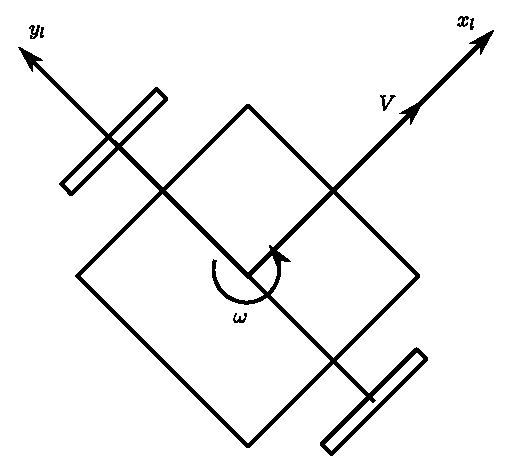
\includegraphics[scale=1]{images/imagess/2lit-DDWMR.eps} 
	\caption{Differential Drive Wheel Mobile Robot}
	\label{fig:Differential Drive Wheel Mobile Robot}
\end{figure}
% Figure Image =============================================================================

\hspace{1.27cm}
Differential drive mobile robot pose is represented in the 2D Cartesian coordinate system. There are two coordinate frames that the robot uses, the global frame and the local frame. In kinematic, the robot velocity is described using two variables and vice versa it is used to control input to the robot. The variables are:\par

\begin{itemize}
\item \(V\), the linear velocity along the x-axis of the local coordinate frame
\item \(\omega\), the angular velocity about the z-axis of the local coordinate frame.
\end{itemize}






\break
\subsection{Controller}
\hspace{1.27cm}
The differential drive mobile robot is a nonholonomic constraint system due to the absence of the velocity along the Y-axis of the local frame. 
The nonholonomic constraint of the robot is:
\begin{equation}
-\Dot{x} sin\theta + \Dot{y} cos\theta = 0
\end{equation}

\textbf{\figureautorefname{ \ref{fig:Mobile Robot Navigation}}} shows a common navigation of mobile robot. To achieve the control of the nonholonomic constraint system, the use of a nonsmooth or time varying controller is needed because the system is nonlinear and varies in time. The robot system is divided into kinematic control and dynamics control. The Most commonly used controls for mobile robots are:
\begin{itemize}
\item \textbf{Control to reference pose}\\
is the control approach where the reference position and orientation is predefined. From the current pose to the reference pose, the robot can drive in an arbitrary path.
\item \textbf{Control to segment of line}\\
is the control approach where the reference segment of the line is constructed from multiple reference poses.
\item \textbf{Control to reference trajectory}\\
is the control approach where the reference pose is a function of time. 
\end{itemize}
\par 

% Figure Image =============================================================================
\begin{figure}[ht]
	\centering
	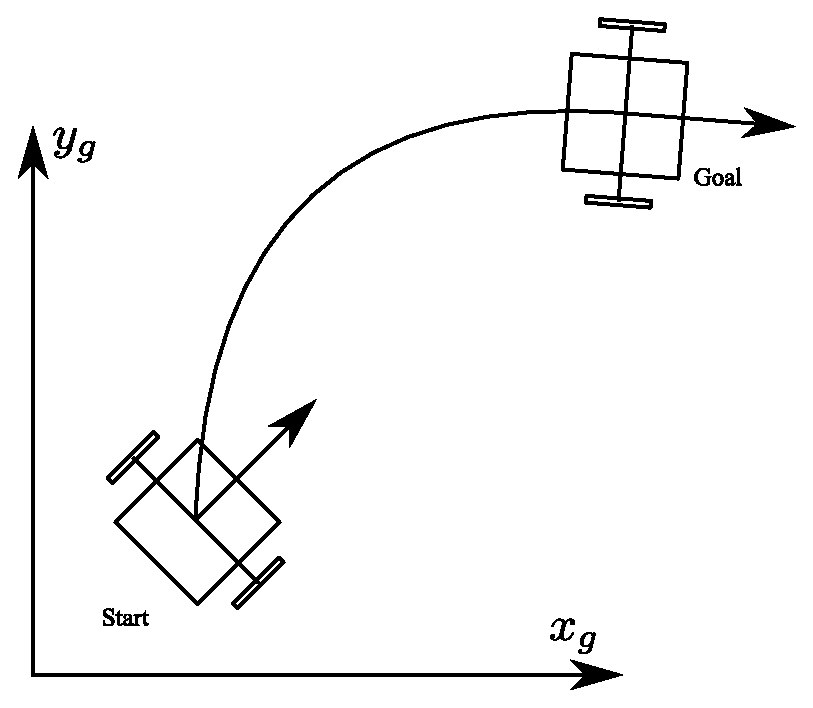
\includegraphics[scale=0.8]{images/imagess/2lit-MRNav.eps} 
	\caption{Mobile Robot Navigation}
	\label{fig:Mobile Robot Navigation}
\end{figure}
% Figure Image =============================================================================

\hspace{1.27cm}
Control wheel mobile robots usually decompose into two part: the \textbf{Feedforward} control and the \textbf{Feedback} control as illustrated in \textbf{\figureautorefname{ \ref{fig:Simple Feedforward and Feedback control}}}.
\begin{itemize}
    \item In \textbf{Feedforward} control, the input to control robot is determined from the calculation of the reference goal or trajectory. The input can then apply to the robot system to move along in the open-loop system.
    \item On the other hand, the \textbf{Feedback} control determine the current state of the robot in every time step and feeds back to the controller for a robust performance.
\end{itemize}
\par

% Figure Image =============================================================================
\begin{figure}[ht]
	\centering
	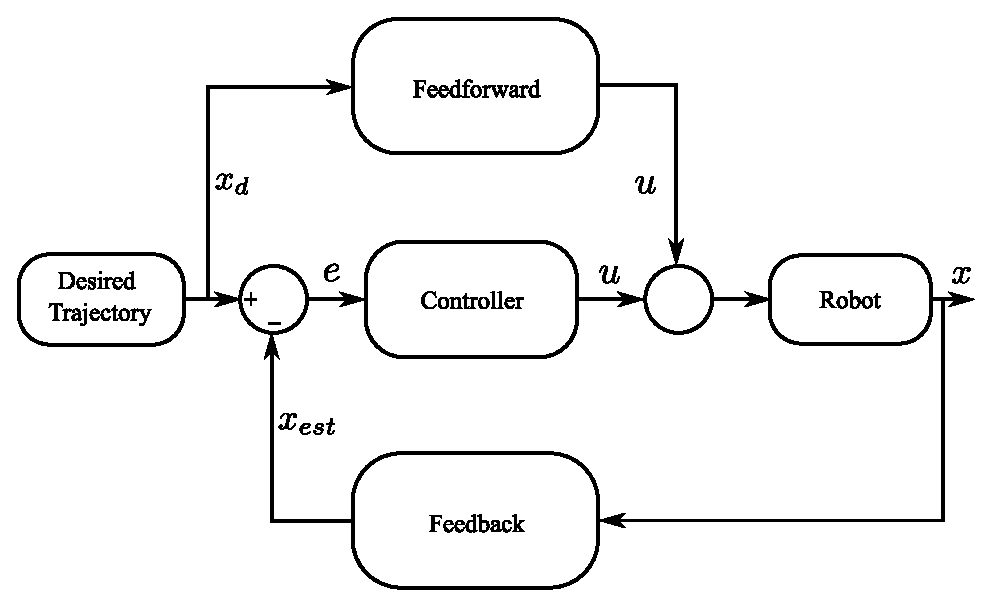
\includegraphics[scale=1]{images/imagess/2lit-simplecontrl.eps} 
	\caption{Simple Feedforward and Feedback control}
	\label{fig:Simple Feedforward and Feedback control}
\end{figure}
% Figure Image =============================================================================

\hspace{1.27cm}
In the real world, the mobile robot is a dynamics system. Thus, for robust control on the dynamics system, the dynamic properties of the system are included, such as torque, mass, moment of inertia, external force acting on the robot,-etc.\\
The controller of the robot dynamics system can be decomposed into two parts: the \textbf{Outer} controller and the \textbf{Inner} controller.
\begin{itemize}
    \item For the \textbf{outer} controller, the system calculate the required system velocities to move along the reference trajectory or to move to a reference pose. 
    \item While the \textbf{inner} control is calculating the torque or force that is required to match the required system velocity from the outer controller.
\end{itemize}
\par














\subsection{Path Planning}

% Figure Image =============================================================================
\begin{figure}[ht]
	\centering
	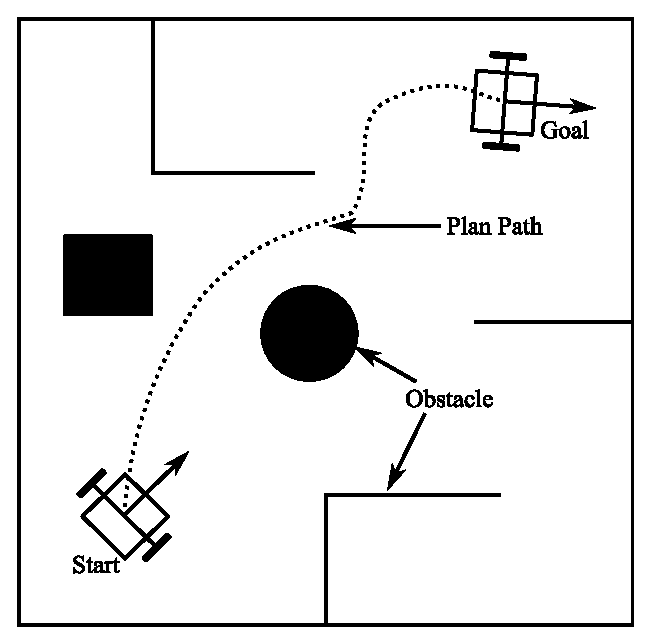
\includegraphics[scale=1]{images/imagess/2lit-pathplan.eps} 
	\caption{Path Planning}
	\label{fig:Path Planning}
\end{figure}
% Figure Image =============================================================================

\hspace{1.27cm}
To reach a certain goal, the robot required a number of information and algorithms to perform. In the process of path planning, the robot computes sequence of valid actions of the robot configuration to move to the goal. In the case of a mobile robot, the problem is usually defined as the moving from start to goal while avoiding the obstacle \textbf{\figureautorefname{ \ref{fig:Path Planning}}}. In the process of path planning of the real world scenario, the robot’s kinematic and dynamic constraints is considered. Since the environment is not always the same, the path planning works with the limited of the representation of the environment in the algorithm. The algorithm can perform in a fully or partly known environment.\par

\hspace{1.27cm}
A preliminary literature review show that there are many approaches to the problem. For example:

$\bullet$ \textbf{Probabilistic Road Maps (PRMs)}

\begin{itemize}
    \item \textbf{Random Space Sampling}\\
    the algorithm indicates the random points in space that are selected to construct a graph, whose edges are created if two nodes abstain no more than a certain distance.\\
    \item \textbf{Space Sampling with Halton Sequence}\\
    a graph is created by selecting points in space using Halton sequence.
    \item \textbf{Uniform Space Sampling}\\
    the algorithm selects even points in the free space at a certain step. Each selected node is connected to eight peripheral sampling points.
\end{itemize}

$\bullet$ \textbf{Visibility Graph}\par
Visibility graph construction is based on the environment's convex obstacles as the algorithm treats their edges as possible nodes. A Ray Casting technique is utilized in order for the robot to perceive the obstacles' edges. As ray detection method has not been expanded as much as the others, the ending point is stored as an obstacle edge, which is the node in the graph. When one node can connect to the other without the graph's edge intersecting an obstacle, the nodes' connections in graph is established.

$\bullet$ \textbf{Rapidly exploring Random Trees — RRTs}
\begin{itemize}
    \item \textbf{Standard RRT}\\
    a random point in the free space is selected. Then, the current constructed tree is checked in order for its closest node to the random point in free space to be found.
    \item \textbf{Star RRT}\\
    the algorithm aim to improve the method of Standard RRT due to highly random path.
    \item \textbf{Multiple RRTs}\\
    the algorithm aim to speed the convergence of Standard RRT
\end{itemize}

$\bullet$ \textbf{Generalized Voronoi Diagram}\par
Generalized Voronoi Diagram is constructed by a set of points in the free space which abstain evenly from the environment's obstacle if the Manhattan distance is taken into account as metric. \par

$\bullet$ \textbf{A* Planning}\par
the algorithm determines the path based on the path cost and cost estimation required to extend the path until the goal using the cost function.\par

Each of the algorithms has their own advantages and disadvantages considered on the computation time and robustness.(\cite{duchovn2014path}) (\cite{inproceedings})
\par

%\break
%\hspace{1.27cm}
%The path planning algorithm introduce the concept of configuration and configuration space. Configuration represents the state of the system in the environment space in n dimension. The state vector is described by $q = [q_1,...,q_n]^T$.The state q is a point in n-dimensional space called configuration space Q, which presents all possible configurations of the mobile system according to its kinematic model. Part of the configuration space that is occupied by the obstacles $O_i$ is denoted $Q_{obst} = \cup_i O_i $. Thus, the part of the environment is \[Q_{free} = Q - Q_{obst}\]
	\section{RESEARCH METHODOLOGY}
\hspace{1.27cm}
The experiment of path planning and control for the mobile robot consists of many steps. First, the mobile robot model and sensor model are built to use inside the simulation software. Second, using the ROS packages Hector SLAM and Gmapping SLAM, the occupancy grid map is built. Third, after the occupancy grid map is built, the A* path planning algorithm is applied to get the trajectory from the start point to the goal point. Finally, the robot movement is controlled to the reference trajectory using backstepping controller algorithm and tuning parameters for smooth motion. \textbf{\figureautorefname{ \ref{fig:Workflow}}} presents the overall workflow of the project.\par

% Figure Image =============================================================================
\begin{figure}[ht]
	\centering
	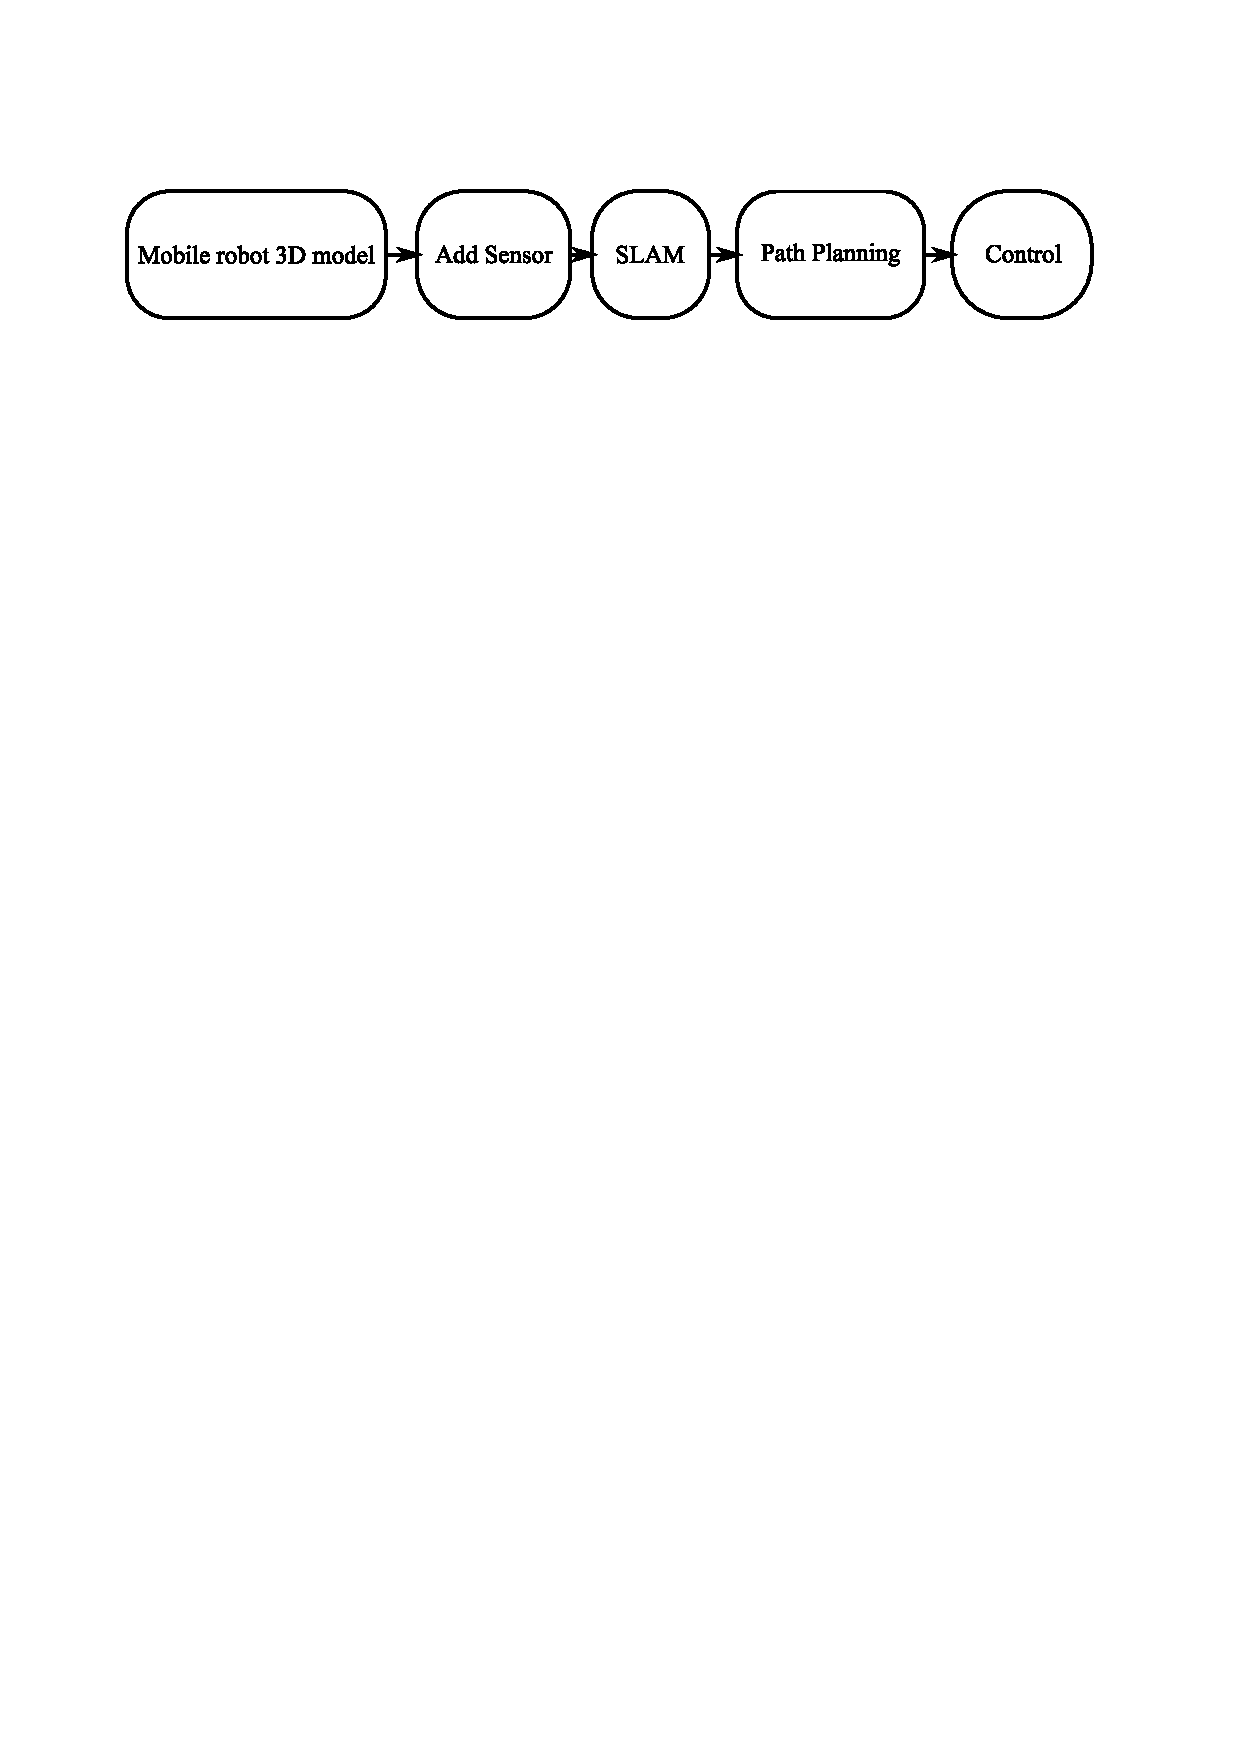
\includegraphics[scale=1]{images/imagess/3method-workflow.pdf}
	\caption{Workflow}
	\label{fig:Workflow}
\end{figure}
% Figure Image =============================================================================

\subsection{Mobile Robot 3D Modelling}
\hspace{1.27cm}
The robot model in constructed in Gazebo simulation. Gazebo uses the robot model written in SDF format. We construct the robot model with the parameters below: \par

$\bullet$ \textbf{Robot Base} (\textbf{\figureautorefname{ \ref{fig:Mobile Robot Base}}})\par
The model base dimensions are:
\begin{itemize}
	\item {\makebox[2cm]{Length\hfill} = 0.4 $m$}
	\item {\makebox[2cm]{Width\hfill} = 0.2 $m$}
	\item {\makebox[2cm]{Height\hfill} = 0.1 $m$}
%    \item Length = 0.4$m$
%    \item Width = 0.2$m$
%    \item Height = 0.1$m$
\end{itemize}

% Figure Image =============================================================================
\begin{figure}[ht]
	\centering
	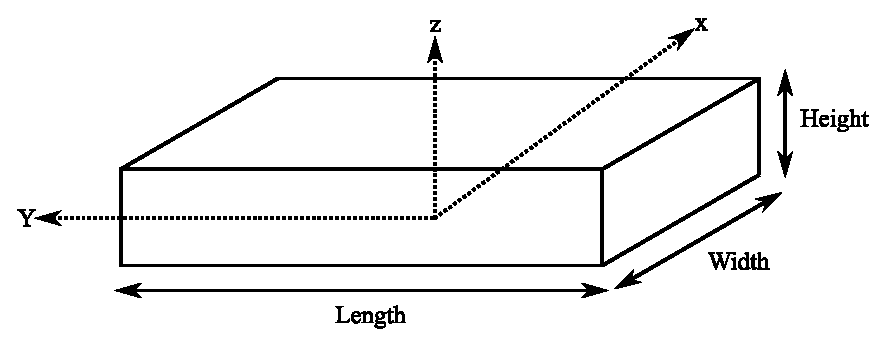
\includegraphics[scale=1]{images/imagess/3method-imu.eps}
	\caption{Mobile Robot Base}
	\label{fig:Mobile Robot Base}
\end{figure}
% Figure Image =============================================================================
\break
$\bullet$ \textbf{Wheels and Caster Wheels} (\textbf{\figureautorefname{ \ref{fig:Mobile Robot Wheel and Caster Wheel}}})\par
The robot wheels and caster wheel dimensions are:
\begin{itemize}
	\item {\makebox[4cm]{Wheel radius\hfill} = 0.1 $m$}
	\item {\makebox[4cm]{Wheel width\hfill} = 0.05 $m$}
	\item {\makebox[4cm]{Caster wheel radius\hfill} = 0.05 $m$}
%    \item Wheel radius = 0.1m
%    \item Wheel width = 0.015m
%    \item Caster wheel radius = 0.25m
\end{itemize}

% Figure Image =============================================================================
\begin{figure}[ht]
	\centering
	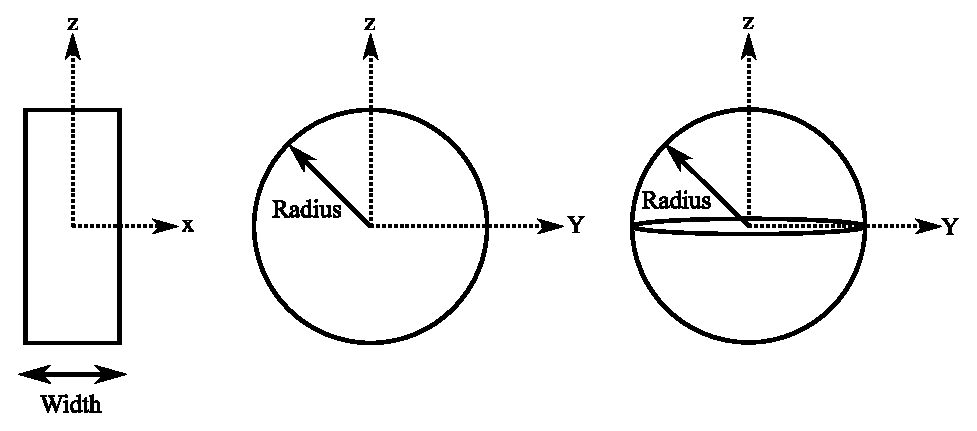
\includegraphics[scale=0.9]{images/imagess/3method-wheel.eps} 
	\caption{Mobile Robot Wheel and Caster Wheel}
	\label{fig:Mobile Robot Wheel and Caster Wheel}
\end{figure}
% Figure Image =============================================================================

\subsection{Sensor 3D Modelling}
\hspace{1.27cm}
The robot is equipped with Lidar sensor, with the max range of 10 $m$, min range of 0.1 $m$, 360$^{\circ}$ field of view, and resolution of 0.1$^{\circ}$. The IMU is attached to the robot frame with the z-axis pointing upward. The sensor noise is included in the simulation with the model of zero-mean Gaussian white. \textbf{\figureautorefname{ \ref{fig:Mobile Robot Modelling Side and Top View}}} illustrates the mobile robot model side and top view.\par

$\bullet$ \textbf{Lidar} (\textbf{\figureautorefname{ \ref{fig:Lidar Dimension}}})\par
The Lidar dimensions are:
\begin{itemize}
	\item {\makebox[3cm]{Diameter\hfill} = 0.065 $m$}
	\item {\makebox[3cm]{Height\hfill} = 0.070 $m$}
	\item {\makebox[3cm]{Height to Laser\hfill} = 0.055 $m$}
%    \item Diameter = 0.1m
%    \item Height = 0.015m
%    \item Height to Laser = 0.25m
\end{itemize}

$\bullet$ \textbf{IMU} (\textbf{\figureautorefname{ \ref{fig:IMU Dimension}}})\par
The IMU dimensions are:
\begin{itemize}
	\item {\makebox[2cm]{Length\hfill} = 0.02 $m$}
	\item {\makebox[2cm]{Width\hfill} = 0.01 $m$}
	\item {\makebox[2cm]{Height\hfill} = 0.01 $m$}
%    \item Length = 0.4m
%    \item Width = 0.2m
%    \item Height = 0.1m
\end{itemize}

% Figure Image =============================================================================
\begin{figure}[ht]
	\centering
	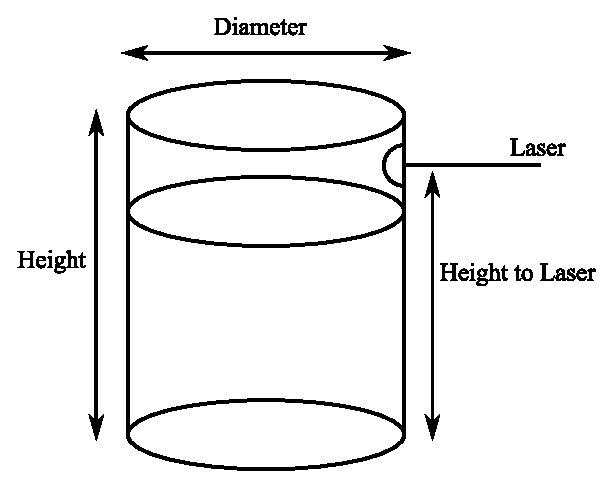
\includegraphics[scale=1]{images/imagess/3method-lidar.eps} 
	\caption{Lidar Dimension}
	\label{fig:Lidar Dimension}
\end{figure}
% Figure Image =============================================================================

% Figure Image =============================================================================
\begin{figure}[ht]
	\centering
	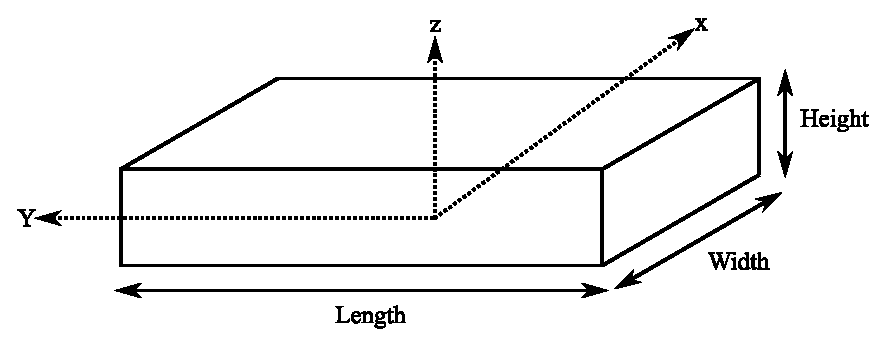
\includegraphics[scale=1]{images/imagess/3method-imu.eps} 
	\caption{IMU Dimension}
	\label{fig:IMU Dimension}
\end{figure}
% Figure Image =============================================================================

% Figure Image =============================================================================
\begin{figure}[H]
	\centering
	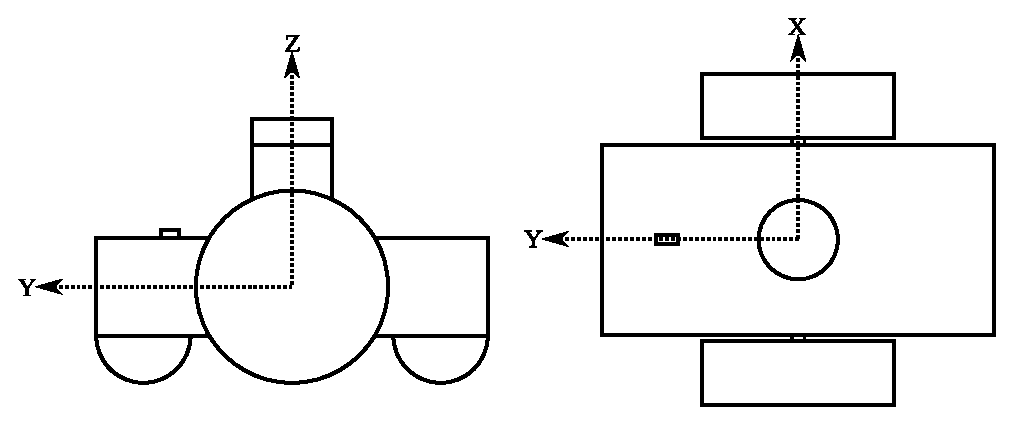
\includegraphics[scale=1]{images/imagess/3method-top-side-view.eps} 
	\caption{Mobile Robot Modelling Side and Top View}
	\label{fig:Mobile Robot Modelling Side and Top View}
\end{figure}
% Figure Image =============================================================================





\subsection{SLAM}
% Figure Image =============================================================================
\begin{figure}[ht]
	\centering
	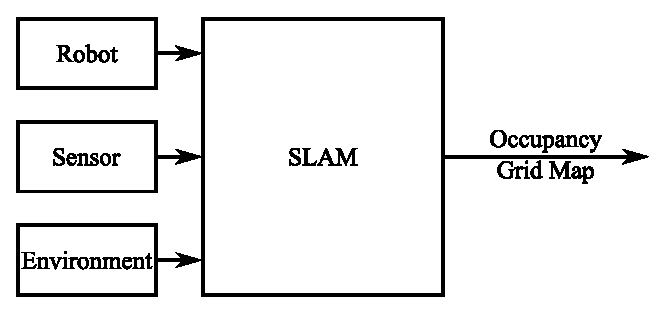
\includegraphics[scale=1]{images/imagess/3method-slam.eps} 
	\caption{SLAM}
	\label{fig:SLAM}
\end{figure}
% Figure Image =============================================================================
\hspace{1.27cm}
\textbf{\figureautorefname{ \ref{fig:SLAM}}}, the SLAM method is used to create the Occupancy Grid Map. In Gazebo, first we create a simulation of the indoor environment. Second, we load the robot model and sensor from the SDF file that is created in the Gazebo. Using ROS plug-in for Gazebo, the robot is controlled with the keyboard input. The robot is driven around while the SLAM is running to create the Occupancy Grid Map of the environment.\par



\subsection{Path Planning and Control}
% Figure Image =============================================================================
\begin{figure}[ht]
	\centering
	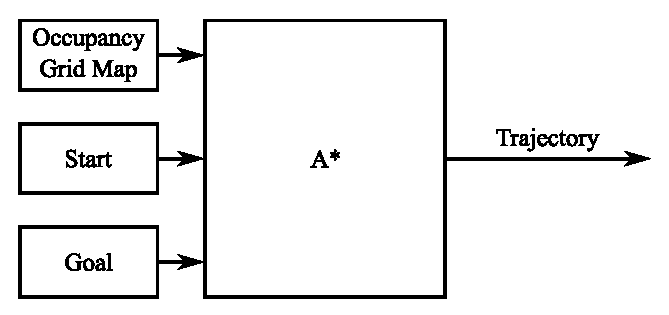
\includegraphics[scale=1]{images/imagess/3method-astar.eps} 
	\caption{Path Planning of Astar}
	\label{fig:Path Planning of Astar}
\end{figure}
% Figure Image =============================================================================
\hspace{1.27cm}
\textbf{\figureautorefname{ \ref{fig:Path Planning of Astar}}}, given the Occupancy Grid Map, the path planning algorithm is used for the calculation of  the reference trajectory for the robot to move. The reference trajectory then is given to the robot which is controlled by the backstepping trajectory tracking algorithm. The control input from the backstepping is publishing on to the ROS control topic to determine the torque of each wheel of the robot to move. In every time-step, the robot pose is estimate using the extended kalman filter sensor fusion algorithm. The pose of the robot is plotted against the reference pose.\par


\hspace{1.27cm}
\textbf{\figureautorefname{ \ref{fig:Map1}}} and \textbf{\figureautorefname{ \ref{fig:Map2}}} are the model of simulated rooms for experiment and its dimension. In this research, we use 2 simulated room model and named it: "Map1" and "Map2". In these 2 figures, the yellow spot represents the Start location for the robot, the green spot represents the goal location where the robot will move to.\\
$\bullet$ \textbf{Indoor 3D models: "Map1"}\par
% Figure Image =============================================================================
\begin{figure}[H]
	\centering
	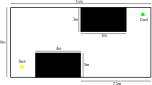
\includegraphics[scale=1]{images/imagess/3method-map1.pdf} 
	\caption{"Map1" Model}
	\label{fig:Map1}
\end{figure}
% Figure Image =============================================================================

$\bullet$ \textbf{Indoor 3D models: "Map2"}\par
% Figure Image =============================================================================
\begin{figure}[H]
	\centering
	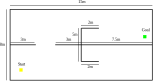
\includegraphics[scale=1]{images/imagess/3method-map2.pdf} 
	\caption{"Map2" Model}
	\label{fig:Map2}
\end{figure}
% Figure Image =============================================================================
	\section{DIFFERENTIAL DRIVE MOBILE ROBOT MODELING}
\subsection{Mobile Robot Kinematic}
\hspace{1.27cm}
Kinematic model of the robot describes the transformation of the robot velocities in the local frame to the velocity in global frame. Using kinematic model, the robot pose is determined and represented in the coordinate system.
\par

% Figure Image =============================================================================
\begin{figure}[ht]
	\centering
	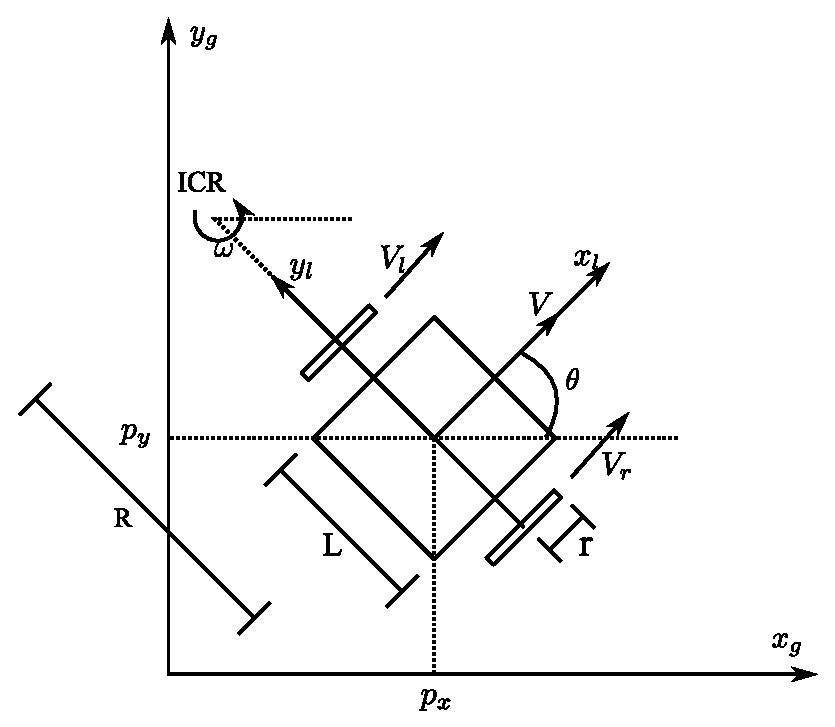
\includegraphics[scale=1]{images/imagess/4dmodel-DDmodeling.eps} 
	\caption{Differential Drive Kinematic Model}
	\label{fig:Differential Drive Kinematic Model}
\end{figure}

% Figure Image =============================================================================
In \textbf{\figureautorefname{ \ref{fig:Differential Drive Kinematic Model}}} Let:
\begin{itemize}
	\item {\makebox[1cm]{\(r\)\hfill} is the radius of the wheel}
	\item {\makebox[1cm]{\(R(t)\)\hfill} is the instantaneous radius of the vehicle driving trajectory}
	\item {\makebox[1cm]{L\hfill} is the length of the robot base}
	\item {\makebox[1cm]{\(V_l\)\hfill} is the linear velocity of the left wheel}
	\item {\makebox[1cm]{\(V_r\)\hfill} is the linear velocity of the right wheel}
	\item {\makebox[1cm]{\(V\)\hfill} is the linear velocity of the robot base}
	\item {\makebox[1cm]{\(\omega\)\hfill} is the angular velocity of the robot base}
	
%	\item \(r\) is the radius of the wheel
%	\item \(R(t)\) is the instantaneous radius of the vehicle driving trajectory
%	\item L is the length of the robot base
%	\item \(V_l\) is the linear velocity of the left wheel
%	\item \(V_r\) is the linear velocity of the right wheel
%	\item \(V\) is the linear velocity of the robot base
%	\item \(\omega\) is the angular velocity of the robot base
\end{itemize}

From \textbf{\figureautorefname{ \ref{fig:Differential Drive Kinematic Model}}}, we obtain:
\begin{equation} \label{eq:MRKi1}
\omega = \frac{V_l(t)}{R(t)-\frac{L}{2}}
\end{equation}
\begin{equation} \label{eq:MRKi2}
\omega = \frac{V_r(t)}{R(t)+\frac{L}{2}}
\end{equation}
\par

From \ref{eq:MRKi1} and \ref{eq:MRKi2}, we get:
\begin{equation} \label{eq:MRKi3}
\omega(t) = \frac{V_r(t)-V_l(t)}{L}
\end{equation}
\begin{equation} \label{eq:MRKi4}
R(t) = \frac{L}{2} \frac{V_r(t)+V_l(t)}{V_r(t)-V_l(t)}
\end{equation}

We have:
\begin{equation} \label{eq:MRKi5}
V(t) = R(t)\omega(t)
\end{equation}

Substitute \ref{eq:MRKi3} and \ref{eq:MRKi4} to \ref{eq:MRKi5}, we get:
\begin{equation}
V(t) = \frac{V_r(t)+V_l(t)}{2}
\end{equation}


We know:
\begin{equation}
\begin{split} \label{eq:MRKi6}
V_l(t) = r\omega_l(t)\\
V_r(t) = r\omega_r(t)
\end{split}
\end{equation}

Substitute \ref{eq:MRKi6} to \ref{eq:MRKi5} and \ref{eq:MRKi3}, we get:
\begin{equation} \label{eq:MRKi_V}
V(t) = \omega_r \frac{r}{2} + \omega_l \frac{r}{2}
\end{equation}
\begin{equation} \label{eq:MRKi_omega}
\omega(t) = \omega_r \frac{r}{L} - \omega_l \frac{r}{L}
\end{equation}


Robot kinematic model in global frame is defined as:
\begin{equation} \label{eq:MRKi7}
\begin{bmatrix}
\Dot{p_x} \\
\Dot{p_y} \\
\Dot{\theta}
\end{bmatrix} = 
\begin{bmatrix}
cos(\theta) && 0\\
sin(\theta) && 0\\
0 && 1
\end{bmatrix}
\begin{bmatrix}
V(t)\\
\omega(t)
\end{bmatrix}
\end{equation}

Using Euler integration, the equation of motion in discrete time form is:
\begin{equation}
\begin{bmatrix}
p_{x,k}\\
p_{y,k}\\
\theta_{k}\\
\end{bmatrix}=
\begin{bmatrix}
p_{x,k-1} + V_{k-1} T_s cos(\theta_{k-1}) \\
p_{y,k-1} + V_{k-1} T_s sin(\theta_{k-1}) \\
\theta_{k-1} + \omega_{k-1} T_s\\
\end{bmatrix}
\end{equation}
Where:
\begin{itemize}
	\item {\makebox[1cm]{k\hfill} is the time step}
	\item {\makebox[1cm]{\(T_s\)\hfill} is the time interval}
%    \item k is the time step
%    \item \(T_s\) is the time interval
\end{itemize}




\subsection{Mobile Robot Dynamics}
\hspace{1.27cm}
Differential drive mobile robot is a dynamics system. Using solely the kinematic model of the system is not enough to represent the system as a whole. For the robustness of the robot, the dynamics properties of the system such as external force, mass, inertia are considered. In our case the robot center of mass is coincides with the center geometric of the robot. Let \(m\) be the mass of the robot, \(J\) be the moment of inertia of the robot about Z-axis. In this section, we use q to describe the generalized coordinate of the system \(q=[x, y, \theta]\) and \(\tau_l\) is the left wheel torque, \(\tau_r\) is the right wheel torque.\par

The dynamics model of the robot with constraint is derived using Lagrange formulation:
\begin{equation}{\label{eq:lagrangain eq full}}
\frac{\partial}{\partial t}(\frac{\partial \mathcal{L}}{\partial \Dot{q}_k})- \frac{\partial \mathcal{L}}{\partial q_k} + \frac{\partial P}{\partial \Dot{q}_k} + g_k + \tau_{dk}= f_k - \sum_{j=1}^{m}\lambda_j a_{jk}
\end{equation}
Where:
\begin{itemize}
	\item {\makebox[1cm]{\(\mathcal{L}\)\hfill} is the Lagrangian}
	\item {\makebox[1cm]{\(P\)\hfill} is the power dissipation function due to friction and damping}
	\item {\makebox[1cm]{\(g_k\)\hfill} are the forces due to gravitation}
	\item {\makebox[1cm]{\(\tau_{dk}\)\hfill} are the system disturbances}
	\item {\makebox[1cm]{\(f_k\)\hfill} are the general forces (external influences to the system)}
	\item {\makebox[1cm]{\(q_k\)\hfill} general coordinate k=(1,...,n)}
	\item {\makebox[1cm]{m\hfill} is the number of linearly independent motion constraint}
	\item {\makebox[1cm]{\(\lambda_j\)\hfill} is the Lagrange multiplier associated with the jth constraint relation}
	\item {\makebox[1cm]{\(a_{jk}\)\hfill} is coefficients of the constraints (j=1,...,n)}
	
%    \item \(\mathcal{L}\) is the Lagrangian
%    \item \(P\) is the power dissipation function due to friction and damping
%    \item \(g_k\) are the forces due to gravitation
%    \item \(\tau_{dk}\) are the system disturbances
%    \item \(f_k\) are the general forces (external influences to the system)
%    \item \(q_k\) general coordinate k=(1,...,n)
%    \item m is the number of linearly independent motion constraint
%    \item \(\lambda_j\) is the Lagrange multiplier associated with the jth constraint relation
%    \item \(a_{jk}\) is coefficients of the constraints (j=1,...,n)
\end{itemize}

Assumption:
\begin{itemize}
	\item {\makebox[1cm]{\(\mathcal{W}_p\)\hfill} = 0, the robot is driven on the plane where the potential energy is constant}
	\item {\makebox[1cm]{\(gk\)\hfill} = 0, the robot is driven on the plane where the potential energy is constant}
	\item {\makebox[1cm]{\(\tau_{dk}\)\hfill} = 0, no outside disturbances}
	
%    \item \(\mathcal{W}_p = 0\), the robot is driven on the plane where the potential energy is constant
%    \item \(gk = 0\), the robot is driven on the plane where the potential energy is constant
%    \item \(\tau_{dk}=0\), no outside disturbances
\end{itemize}

The Lagrangian \(\mathcal{L}\) is the difference between kinetic energy and potential energy. We get:
\begin{equation}
\mathcal{L} = \mathcal{W}_k - \mathcal{W}_p 
\end{equation}
Where:
\begin{itemize}
	\item {\makebox[1cm]{\(\mathcal{W}_k\)\hfill} is the kinetic energy of the system}
	\item {\makebox[1cm]{\(\mathcal{W}_p\)\hfill} is the potential energy of the system}
	
%    \item \(\mathcal{W}_k\) is the kinetic energy of the system
%    \item \(\mathcal{W}_p\) is the potential energy of the system
\end{itemize}

The Kinetic energy equation is:
\begin{equation}
\mathcal{W}_k = \frac{1}{2}mV^2 + \frac{1}{2} J\Dot{\theta}^2
\end{equation}

The velocity in the 2D plane is:
\begin{equation}
V^2 = \Dot{x}^2 + \Dot{y}^2
\end{equation}

We get the Lagrangian \(\mathcal{L}\):
\begin{equation}
\mathcal{L} = \frac{m}{2}(\Dot{x}^2 + \Dot{y}^2) + \frac{J}{2}\Dot{\theta}^2
\end{equation}

Substitute back to \ref{eq:lagrangain eq full}, we get:
\[\frac{\partial}{\partial t}(\frac{\partial \mathcal{L}}{\partial \Dot{x}}) = m\Ddot{x}\] 
\[\frac{\partial}{\partial t}(\frac{\partial \mathcal{L}}{\partial \Dot{y}}) = m\Ddot{y}\] 
\[\frac{\partial}{\partial t}(\frac{\partial \mathcal{L}}{\partial \Dot{\theta}}) = J\Ddot{\theta}\]
\[\frac{\partial \mathcal{L}}{\partial x} = 0\] 
\[\frac{\partial \mathcal{L}}{\partial y} = 0\] 
\[\frac{\partial \mathcal{L}}{\partial \theta} = 0\] 

The mobile robot constraint in x-axis is \(-sin\theta\), in y-axis is \(cos\theta\).\\
From \ref{eq:lagrangain eq full}, we obtain:
\begin{equation}
\begin{split}
m\Ddot{x} = F_x - \lambda_1(-sin\theta) \\
m\Ddot{y} = F_y - \lambda_1(cos\theta)\\
J\Ddot{\theta} = M_z
\end{split}
\end{equation}

We get:
\begin{equation}
\begin{split}
m\Ddot{x} - \lambda_1 sin \theta= F_x\\
m\Ddot{y} + \lambda_1 cos \theta= F_y\\
J\Ddot{\theta} = M_z
\end{split}
\end{equation}

Since the assumption of no outside disturbance force, the force acting on the robot are the left wheel force \(F_l\) and the right wheel force \(F_r\). The resultant for is:
\begin{equation}
F = F_r + F_l
\end{equation}

We have:
\begin{equation}
\begin{split}
F_r = \frac{\tau_r}{r}\\
F_l = \frac{\tau_l}{r}
\end{split}
\end{equation}

And
\begin{equation}
\begin{split}
F_x &= F cos\theta \\
F_y &= F sin\theta \\
M_z &= F_r \frac{L}{2} - F_l \frac{L}{2}
\end{split}
\end{equation}

We get:
\begin{equation}
\begin{split}
F_x &= \frac{1}{r} (\tau_r + \tau_l) cos \theta \\
F_y &= \frac{1}{r} (\tau_r + \tau_l) sin \theta \\
M_z &= \frac{L}{2r} (\tau_r - \tau_l)
\end{split}
\end{equation}

We get:
\begin{equation}
\begin{split}
m\Ddot{x} - \lambda sin \theta - \frac{1}{r} (\tau_r + \tau_l) cos \theta = 0\\
m\Ddot{y} + \lambda cos \theta - \frac{1}{r} (\tau_r + \tau_l) sin \theta = 0\\
J\Ddot{\theta} - \frac{L}{2r} (\tau_r - \tau_l) = 0
\end{split}
\end{equation}

Rewrite the equation into Matrix form of:
\[M(q)\Ddot{q} + V (q,\Dot{q}) + F(\Dot{q}) = E(q)u - A^T(q) \lambda\]
We get:
\[M=\begin{bmatrix}
m && 0 && 0\\
0 && m && 0\\ 
0 && 0 && J
\end{bmatrix}\]

\[E=\frac{1}{r}\begin{bmatrix}
cos\theta && cos\theta \\
sin\theta && sin\theta \\ 
\frac{L}{2} && -\frac{L}{2} 
\end{bmatrix}\]

\[A=\begin{bmatrix}
-sin\theta && cos\theta && 0
\end{bmatrix}\]

\[u=\begin{bmatrix}
\tau_r\\
\tau_l 
\end{bmatrix}\]

Where remain are Zero\newline
In the state-space model:

\[\Tilde{M}=\begin{bmatrix}
m && 0 \\
0 && j
\end{bmatrix}\]

\[\Tilde{V}=\begin{bmatrix}
0\\
0
\end{bmatrix}\]

\[\Tilde{E}=\frac{1}{r}\begin{bmatrix}
1 && 1 \\
\frac{L}{2} && -\frac{L}{2} \\ 
\end{bmatrix}\]

The model is
\begin{equation}
\begin{bmatrix}
\Dot{x}\\
\Dot{y}\\
\Dot{\theta}\\
\Dot{V}\\
\Dot{\omega}
\end{bmatrix}=
\begin{bmatrix}
V cos\theta\\
V sin\theta\\
\omega\\
0\\
0
\end{bmatrix}+
\begin{bmatrix}
0&& 0 \\
0&& 0 \\
0&& 0 \\
\frac{1}{mr}&& \frac{1}{mr} \\
\frac{L}{2Jr}&&-\frac{L}{2Jr}
\end{bmatrix}\begin{bmatrix}
\tau_r\\
\tau_l
\end{bmatrix}
\end{equation}

%Using Inverse Model gives the required torque for each wheel to be calculated
%\begin{equation}
%\begin{bmatrix}
%\tau_r\\
%\tau_l
%\end{bmatrix}=
%\begin{bmatrix}
%\frac{\Dot{V}mr}{2} + \frac{\Dot{\omega}Jr}{L}\\
%\frac{\Dot{V}mr}{2} - \frac{\Dot{\omega}Jr}{L}
%\end{bmatrix}
%\end{equation}
	\section{CONTROL DIFFERENTIAL DRIVE MOBILE ROBOT}
\hspace{1.27cm}
There are multiple ways to control the mobile robot, namely, reference position control and reference trajectory control —etc. In this project, the robot movement is control by the trajectory tracking control based on the back-stepping technique.\par
\subsection{Kinematic Control Model}

\hspace{1.27cm}
% Figure Image =============================================================================
\begin{figure}[ht]
	\centering
	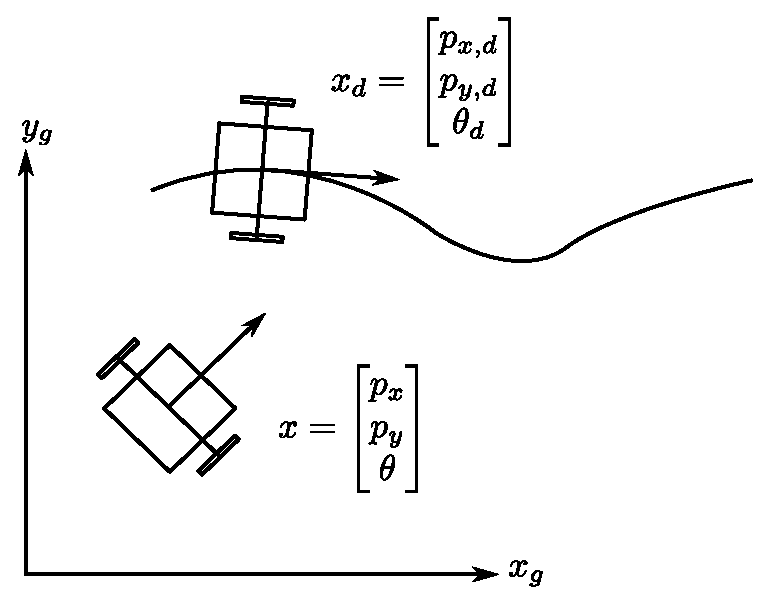
\includegraphics[scale=1]{images/imagess/5cont-kinematic.eps} 
	\caption{Differential Drive Kinematic control}
	\label{fig:Differential Drive Kinematic control}
\end{figure}
% Figure Image =============================================================================

\textbf{\figureautorefname{ \ref{fig:Differential Drive Kinematic control}}} shows the robot pose inside the environment. Let :
\begin{itemize}
	\item {\makebox[1cm]{\(x\)\hfill} represents the current pose of the robot in a time step}
	\item {\makebox[1cm]{\(x_d\)\hfill} represents the desired trajectory of the robot}
	
%    \item \(x\) represents the current pose of the robot in a time step
%    \item \(x_d\) represents the desired trajectory of the robot to move on
\end{itemize}
The purpose of the back-stepping trajectory tracking control controller is to nullify the error between the \(x\) and \(x_d\). The error between the current pose and the desired trajectory pose is defined as:

\begin{equation} \label{eq:control_error}
x_e = T \Tilde{x}
\end{equation}

Where:
\begin{equation}
x_e =
\begin{bmatrix}
e_1\\
e_2\\
e_3
\end{bmatrix}
\end{equation}

\begin{equation}
T = \begin{bmatrix}
cos\theta && sin\theta && 0\\
-sin\theta && cos\theta && 0\\
0 && 0 && 1
\end{bmatrix}
\end{equation}

\begin{equation}
\Tilde{x} = \begin{bmatrix}
p_{x,d} - p_x\\
p_{y,d} - p_y\\
\theta_d - \theta
\end{bmatrix}
\end{equation}

Taking the derivative of \ref{eq:control_error}, we obtain:
\begin{equation}
\Dot{x}_e=
\begin{bmatrix}
\Dot{e}_1\\
\Dot{e}_2\\
\Dot{e}_3
\end{bmatrix}=
\begin{bmatrix}
-1\\
0\\
0
\end{bmatrix}V+
\begin{bmatrix}
e_2\\
-e_1\\
-1
\end{bmatrix}\omega+
\begin{bmatrix}
V_{ref} cos e_3\\
V_{ref} sin e_3\\
\omega_{ref}
\end{bmatrix}
\end{equation}

Proving by the Lyapunov stability (\cite{zidani2015backstepping}), the controllers produce the control input for the robot are:
\begin{equation}
\begin{bmatrix}
V_c\\
\omega_c
\end{bmatrix} = 
\begin{bmatrix}
V_{ref} cos e_3 + k_1e_1\\
\omega_{ref} + k_2 V_{ref} e_2 + k_2 sin e_3
\end{bmatrix}
\end{equation}

Where:
\begin{itemize}
	\item {\makebox[2cm]{\(k_1,k_2,k_3\)\hfill} are the positive constants for tuning}
	\item {\makebox[2cm]{\(V_c\)\hfill} is a linear velocity control}
	\item {\makebox[2cm]{\(\omega_c\)\hfill} is an angular velocity control}
	
%	\item \(k_1,k_2,k_3\) are the positive constants for tuning
%	\item \(V_c\) is a linear velocity control 
%	\item \(\omega_c\) is an angular velocity control
\end{itemize}






\subsection{Dynamics Control Model}
\hspace{1.27cm}
Using the dynamics model of the robot, reformulate in terms of tracking control. By using coordinate transformation. Let:
\begin{equation}
\begin{split}
x_1 &= V\\
x_2 &= \omega\\
u_V &= \tau_1 + \tau_2\\
u_\omega &= \tau_1 - \tau_2
\end{split}
\end{equation}

Where:
\begin{itemize}
	\item {\makebox[2cm]{\((x_1,x_2)^T\)\hfill} is the state vector}
	\item {\makebox[2cm]{\((u_V,u_\omega)^T\)\hfill} is the control vector}
	
%    \item \((x_1,x_2)^T\) is the state vector
%    \item \((u_V,u_\omega)^T\) is the control vector
\end{itemize}

We get:
\begin{equation}
\Dot{x_1} = \frac{1}{mr}u_V
\end{equation}
\begin{equation}
\Dot{x_2} = \frac{L}{2rI}u_\omega
\end{equation}
There are two steps in this approach:\\
$\bullet$ \textbf{Step 1}:\par
Let \(x_{1ref}\) be the linear velocity of the reference trajectory. The linear velocity tracking error is defined as:
\begin{equation}
z_1 = x_{1ref} - x_1
\end{equation}
Taking the derivative of \(z_1\), we get: 
\begin{equation}
\Dot{z}_1 = \Dot{x}_{1ref}-\Dot{x}_1 = \Dot{x}_{1ref} - \frac{1}{mr} u_V
\end{equation}
From the Lyapunov function stability, we get:
\begin{equation} \label{eq:control_uV}
u_V = mr[\Dot{x}_{1ref} + k_az_1]
\end{equation}

\break
$\bullet$ \textbf{Step 2}:\par
Let \(x_{2ref}\) be the angular velocity of the reference trajectory. The angular velocity tracking error is defined as:
\begin{equation}
z_2 = x_{2ref} - x_2
\end{equation}
Taking the derivative of \(z_2\), we get:
\begin{equation}
\Dot{z}_2 = \Dot{x}_{2ref}-\Dot{x}_2 = \Dot{x}_{2ref} - \frac{L}{2rI} u_\omega
\end{equation}
From the Lyapunov function stability, we get:
\begin{equation} \label{eq:control_uomega}
u_\omega = \frac{2rI}{L}[\Dot{x}_{2ref} + k_bz_2]
\end{equation}

We have:
\begin{equation} \label{eq:control tau 1c}
\tau_{1c} = \frac{1}{2}[u_V+u_\omega]
\end{equation}
\begin{equation} \label{eq:control tau 2c}
\tau_{2c} = \frac{1}{2}[u_V-u_\omega]
\end{equation}

Substitute \ref{eq:control_uV} and \ref{eq:control_uomega} into \ref{eq:control tau 1c} and \ref{eq:control tau 2c}, we get:
\begin{equation}
\tau_{1c} = \frac{1}{2}[mr[\Dot{x}_{1ref} + k_az_1]]+\frac{2rI}{L}[\Dot{x}_{2ref} + k_bz_2]]\\
\end{equation}
\begin{equation}
\tau_{2c} = \frac{1}{2}[mr[\Dot{x}_{1ref} + k_az_1]]-\frac{2rI}{L}[\Dot{x}_{2ref} + k_bz_2]]
\end{equation}

Where:
\begin{itemize}
	\item {\makebox[1cm]{\(\tau_{1c}\)\hfill} is the control torque for the left wheel}
	\item {\makebox[1cm]{\(\tau_{2c}\)\hfill} is the control torque for the right wheel}
	\item {\makebox[1cm]{\(k_a\)\hfill} is a positive constant}
	\item {\makebox[1cm]{\(k_b\)\hfill} is a positive constant}
	
%	\item \(\tau_{1c}\) is the control torque for the left wheel
%	\item \(\tau_{2c}\) is the control torque for the right wheel
%	\item \(k_a\) is a positive constant
%	\item \(k_b\) is a positive constant
\end{itemize}






\break
\subsection{Sensor Fusion}
\hspace{1.27cm}
Sensor fusion is the method of combining the data from the sensor to determine the state of the system. One of the sensor fusion algorithms is Kalman Filter. It is an algorithm that estimates of the unknown or uncertain variable given the observation. The state of the system (in this case, the robot pose) is represented as vector with some mixed in noise (considered as ground truth). In every discrete time step, the new state is determined in the function of previous state and inputs using an operator. Then, another operator determines the measurable output (observation) from the true system. This algorithm can only apply to the linear system. Since the mobile robot is a nonlinear system, another variance of Kalman Filter is used called Extended Kalman Filter. (\cite{al2015multiple}) (\cite{moore2016generalized}). The state transition model and the measurement model in EKF are defined as :\par
\begin{equation}
    x_k = f(x_{k-1},u_{k-1}) + w_{k-1}
\end{equation}
\begin{equation}
    y_k = h(x_k) + v_k
\end{equation}

EKF is divided into two steps: the \textbf{Prediction step} and the \textbf{Correction step}.
% Table ====================================================================================
\begin{table}[h]
    \begin{center}
		\caption{Extended Kalman Filter Algorithm (\cite{kim2018introduction})}
		\label{Table: Extended Kalman Filter Algorithm}
		\begin{tabular}{lll}
		\hline
		Prediction                  && \\
		\hline
		Predicted State estimate    && \(\hat{x}^-_k = f(\hat{x}^-_{k-1},u_{k-1})\) \\
		Predicted error co-variance && \(P^-_k = JF_{k-1}P^+_{k-1}JF^T_{k-1} + Q\)\\
		\hline
        Correction                  && \\
        \hline
        Measurement predict         && \(\hat{y}_k = h(\hat{x}^-_k)\)\\
        Measurement residual        && \(\Tilde{y}_k = y_k - \hat{y}_k\)\\
        Kalman Gain                 && \(K_k = P^-_kJH^T_k(R+JH_kP^-_kJH^T_k)^{-1}\)\\
        Updated state estimate      && \(\hat{x}^+_k = \hat{x}^-_k + K_k\Tilde{y}\)\\
        Updated error co-variance   && \(P^+_k = (I-K_kJH_k)P^-_k\)\\
		%\hline
		\ChangeRT{1.5pt} 
       \end{tabular}
  \end{center}
\end{table}
% Table ====================================================================================

The superscript - and + represents the variable prior and posterior to the estimate state in the time update and the measurement update, respectively.

From \textbf{\tableautorefname{ \ref{Table: Extended Kalman Filter Algorithm}}},
\begin{itemize}
	\item {\makebox[1cm]{\(x\)\hfill} is the state vector}
	\item {\makebox[1cm]{\(P\)\hfill} is the error co-variance}
	\item {\makebox[1cm]{\(y\)\hfill} is the measurement vector}
	\item {\makebox[1cm]{\(k\)\hfill} is the time step}
	\item {\makebox[1cm]{\(u\)\hfill} is the control input vector}
	\item {\makebox[1cm]{\(w\)\hfill} is the guassian white noise}
	\item {\makebox[1cm]{\(v\)\hfill} is the guassian white noise }
	\item {\makebox[1cm]{\(Q\)\hfill} is the covariance matrix of prediction model}
	\item {\makebox[1cm]{\(R\)\hfill} is the covariance matrix of measurement model}
	\item {\makebox[1cm]{\(JF_{k-1}\)\hfill} is the Jacobian matrix the nonlinear state function}\\
	\[JF_{k-1} = \frac{\partial f}{\partial x}|_{\hat{x}^+_{k-1},u_{k-1}}\]
	\item {\makebox[1cm]{\(JH_k\)\hfill} is the Jacobian matrix of the nonlinear measurement function}\\
	\[JH_k = \frac{\partial h}{\partial x}|_{\hat{x}^-_k}\]

	
%	\item \(x\) is the state vector
%	\item \(P\) is the error co-variance
%	\item \(y\) is the measurement vector
%	\item \(k\) is the time step
%	\item \(u\) is the control input vector
%	\item \(w\) is the guassian white noise 
%	\item \(v\) is the guassian white noise
%	\item \(Q\) is the covariance matrix of prediction model
%	\item \(R\) is the covariance matrix of measurement model
%	\item \(JF_{k-1}\) is the Jacobian matrix the nonlinear state function\\
%	\[JF_{k-1} = \frac{\partial f}{\partial x}|_{\hat{x}^+_{k-1},u_{k-1}}\]
%	\item \(JH_k\) is the Jacobian matrix of the nonlinear measurement function\\
%	\[JH_k = \frac{\partial h}{\partial x}|_{\hat{x}^-_k}\]
\end{itemize}


$\bullet$ \textbf{Overall sensor fusion localization}\par
\hspace{1.27cm}
Using EKF, the robot pose \(x = [p_x\quad p_y\quad \theta]^T\) is predicted and estimated. In the \textbf{Prediction step}, from the wheel encoder signal the \(V\) and the \(\omega\) are calculated and subsequently are used to predict the robot state \(\hat{x}_k^-\) and the error covariance \(P_k^-\). In the \textbf{Correction step}, the robot pose \([p_x\quad p_y]\) is measured from the Scan Matching Lidar, and the robot orientation \([\theta]\) is measured from the continuously integrated angular velocity \(\omega\) of the IMU.\par

$\bullet$ \textbf{Prediction Step}\par
In state space representation, the system is defined as:
\begin{equation} \label{eq:control1}
x_k = F x_{k-1} + B u_{k-1}
\end{equation}
Where:
\begin{itemize}
	\item {\makebox[1cm]{F\hfill} is the state transition matrix}
	\item {\makebox[1cm]{B\hfill} is the control input matrix}
	\item {\makebox[1cm]{\(x\)\hfill} is the state vector}
	\item {\makebox[1cm]{\(u\)\hfill} is the control input vector}

%	\item F is the state transition matrix
%	\item B is the control input matrix
%	\item \(x\) is the state vector
%	\item \(u\) is the control input vector
\end{itemize}

\break
$\bullet$ Wheel Encoder\par
Wheel encoder signal \(\omega_l\) and \(\omega_r\) are used to calculate the \(u\) and \(x\).\\ We have:
\begin{equation}
u_{k-1} = 
\begin{bmatrix}
V_{k-1}\\
\omega_{k-1}
\end{bmatrix}
\end{equation}

And

\begin{equation}
\begin{bmatrix}
V\\
\omega
\end{bmatrix}=\begin{bmatrix}
\frac{r}{2} & \frac{r}{2}\\
\frac{r}{L} & -\frac{r}{L}
\end{bmatrix}\begin{bmatrix}
\omega_r\\
\omega_l
\end{bmatrix}
\end{equation}


Rewrite the \ref{eq:MRKi7}, into the state space representation as the \ref{eq:control1} form, we have:
\begin{equation}
\begin{bmatrix}
p_{x,k}\\
p_{y,k}\\
\theta_k
\end{bmatrix}=\begin{bmatrix}
1 & 0 & 0\\
0 & 1 & 0\\
0 & 0 & 1
\end{bmatrix}\begin{bmatrix}
p_{x,k-1}\\
p_{y,k-1}\\
\theta_{k-1}
\end{bmatrix}+\begin{bmatrix}
cos(\theta_{k-1}) T_s && 0\\
sin(\theta_{k-1}) T_s && 0\\
0 && T_s
\end{bmatrix}
\begin{bmatrix}
V_{k-1}\\
\omega_{k-1}
\end{bmatrix}
\end{equation}

We get:
\begin{equation}
F = \begin{bmatrix}
1 & 0 & 0\\
0 & 1 & 0\\
0 & 0 & 1
\end{bmatrix}
\end{equation}
\begin{equation}
B = \begin{bmatrix}
cos(\theta_{k-1}) T_s && 0\\
sin(\theta_{k-1}) T_s && 0\\
0 && T_s
\end{bmatrix}
\end{equation}


$\bullet$ Jacobian Matrix JF\par
From \ref{eq:MRKi7}, we have:
\begin{equation} \label{eq:control2}
\begin{split}
\Dot{p_x} &= V cos \theta\\
\Dot{p_y} &= V sin \theta\\
\Dot{\theta} &= \omega
\end{split}
\end{equation}

We have:
\begin{equation} \label{eq:control3}
Jacobian = \begin{bmatrix}
\frac{\partial p_x}{\partial p_x} & \frac{\partial p_x}{\partial p_y} & \frac{\partial p_x}{\theta}\\
\frac{\partial p_y}{\partial p_x} & \frac{\partial p_y}{\partial p_y} & \frac{\partial p_y}{\theta}\\
\frac{\partial \theta}{\partial p_x}       & \frac{\partial \theta}{\partial p_y}       & \frac{\partial \theta}{\partial \theta}
\end{bmatrix}
\end{equation}

Substitute \ref{eq:control2} into \ref{eq:control3}, we get the Jacobian Matrix of F (JF):
\begin{equation}
JF = 
\begin{bmatrix}
1 & 0 & -V_{k-1} T_s sin(\theta_{k-1})\\
0 & 1 &  V_{k-1} T_s cos(\theta_{k-1})\\
0 & 0 &            1
\end{bmatrix}
\end{equation}

$\bullet$ \textbf{Correction Step}\par
The measurement prediction:
\begin{equation}
\hat{y}_k = H x_k
\end{equation}
Where
\begin{equation}
H = \begin{bmatrix}
1 & 0 & 0\\
0 & 1 & 0\\
0 & 0 & 1
\end{bmatrix}
\end{equation}

$\bullet$ Sensor Correction Measurement \(y_k\)\par
$\bullet$ Lidar\par
Lidar measures distances and angles to the obstacle. From Scan Matching Lidar, the robot pose \(p_x,p_y\) is measured. Thus, the measurement model of the Lidar is:
\begin{equation}
\begin{split}
y_{1,k} = p_{x,k}\\
y_{2,k} = p_{y,k}
\end{split}
\end{equation}

$\bullet$ IMU\par
IMU use Gyroscope to measure the angular velocity of the robot. From continuously integrating gyroscope data around Z-axis, the heading angle of the robot is measured. Thus, the measurement model of the IMU is :
\begin{equation}
y_{3,k} = \omega T_s
\end{equation}

$\bullet$ Jacobian Matrix (JH)\par
\begin{equation}
JH = \begin{bmatrix}
1 & 0 & 0\\
0 & 1 & 0\\
0 & 0 & 1
\end{bmatrix}
\end{equation}



\break
\textbf{\figureautorefname{ \ref{fig:Sensor Fusion Localization and control architecture}}} shows the overall Sensor Fusion Localization and Control Architecture of the whole system.
% Figure Image =============================================================================
\begin{figure}[ht]
	\centering
	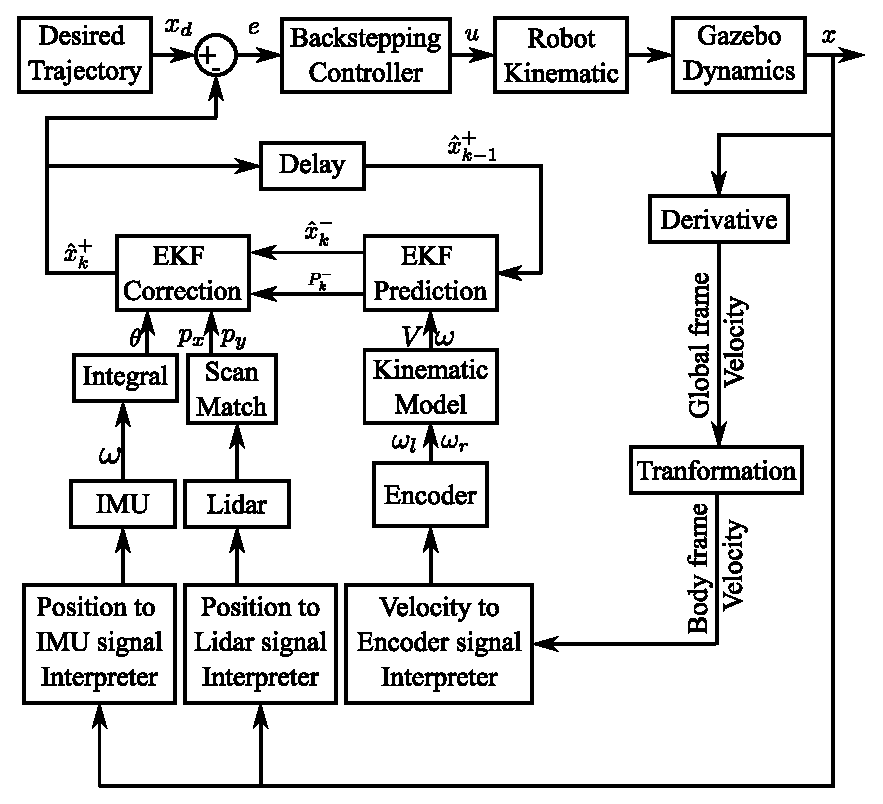
\includegraphics[scale=1]{images/imagess/5cont-propose_arch.eps} 
	\caption{Sensor Fusion Localization and control architecture}
	\label{fig:Sensor Fusion Localization and control architecture}
\end{figure}
% Figure Image =============================================================================
	\section{PATH PLANNING}
\subsection{Robotic Operating System (ROS)}
% Figure Image =============================================================================
\begin{figure}[ht]
	\centering
	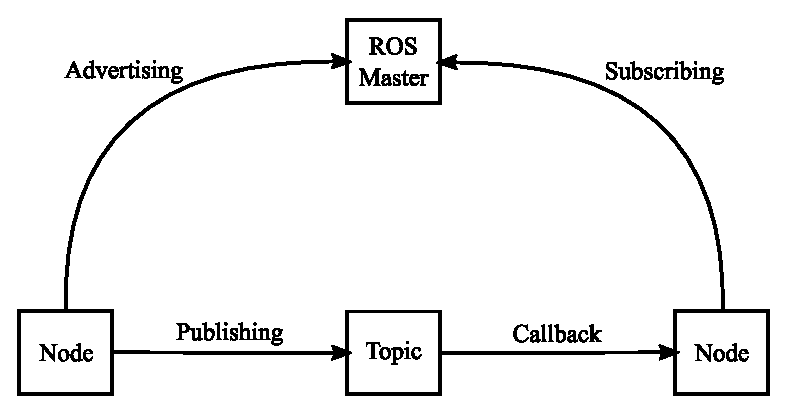
\includegraphics[scale=1]{images/imagess/6pp-ros.eps} 
	\caption{ROS Framework}
	\label{fig:ROS Framework}
\end{figure}
% Figure Image =============================================================================
\hspace{1.27cm}
Robotic operating system (ROS) is an open source framework developed for robotic purposes. It contains libraries and packages that are already built and ready to use for robots. ROS is a peer-to-peer network of processes that could run on multiple devices that are connected via network.(\cite{rosabout})\par
\hspace{1.27cm}
\textbf{\figureautorefname{ \ref{fig:ROS Framework}}}, ROS center of communication is ROS Master. ROS master acts as a keeper of topics and services, registration and information of ROS nodes. ROS nodes are the process of performing the computation. It publishes or subscribes ROS messages with other nodes via ROS topics. ROS message is a data that has been simplified into a structure.\par

\subsubsection{Odometry Message}
\hspace{1.27cm}
Odometry is the information of robot position and velocity within the environment. In 3D coordinate system, the robot position is represented as \([p_x\quad p_y\quad p_z]^T\) and the orientation of the robot is represented as roll, pitch, yaw in Euler angle representation. As our robot is in 2D planar motion, thus we only interested in \([p_x\quad p_y\quad \theta]^T\). When using the ROS message, the odometry directly publishes with the position and orientation of the robot from the simulated environment. The position is expressed as \([p_x\quad p_y]\) and the orientation in the quaternion form \((qw,qx,qy,qz)\).\par
\break
In this project the Odometry Message is used to contain the data of:
\begin{itemize}
	\item Lidar scan matching
	\item Wheel encoder odometry
	\item EKF fusion pose
	\item Robot true pose
	\item Robot current pose
\end{itemize}


% Table ====================================================================================
\begin{table}[ht]
    \begin{center}
		\caption{Odometry Properties (\cite{rosodom})}
		\label{Table: Odometry Properties}
		\begin{tabular}{p{0.4\linewidth}  p{0.5\linewidth}}
		ROS message & Definition \\
		\hline
        Header & Timestamp and frame id \\
        Child frame id &  \\
        Geometry\_msgs/PoseWithCovariance & Estimation of WMR Position in free space with uncertainty\\
        Geometry\_msgs/Pose & Contain the information of the position x,y,z and orientation in quaternion form (x,y,z,w)\\
        Geometry\_msgs/TwistWithCovariance & Estimation of WMR Velocity in free space with uncertainty \\
        Geometry\_msgs/Twist & Contain the information of velocity in linear and angular\\
        %\hline
        \ChangeRT{1.5pt} 
       \end{tabular}
  \end{center}
\end{table}

\textbf{\tableautorefname{ \ref{Table: Odometry Properties}}}, In the ROS Odometry properties, In global frame,\\
$\bullet$ \textbf{Robot poses is:}\par
\begin{itemize}
	\item Odometry.Pose.Pose.Position.x = \(p_x\)
	\item Odometry.Pose.Pose.Position.y = \(p_y\)
	\item Odometry.Pose.Pose.Orientation.(qw,qx,qy,qz) = \(\theta\)
\end{itemize}
$\bullet$ \textbf{Robot velocity is:}\par
\begin{itemize}
	\item Odometry.twist.twist.linear.x = \(\Dot{p_x}\)
	\item Odometry.twist.twist.linear.y = \(\Dot{p_y}\)
	\item Odometry.twist.twist.angular.z = \(\omega\)
\end{itemize}




\subsubsection{IMU Message}
\hspace{1.27cm}
IMU is a module that consists of three different types of sensors (triaxial). Those sensors are accelerometer, gyroscopes, and magnetometer, which measure the acceleration, the angular velocity, and the magnetic field, respectively. The IMU ROS message are used to show the data of velocity, acceleration, and orientation of a system in quaternion form.\par
\break
In this project the IMU Message is used to contain the data of:
\begin{itemize}
	\item Robot Estimated Orientation
	\item Robot linear and angular velocity
\end{itemize}

% Table ====================================================================================
\begin{table}[ht]
    \begin{center}
		\caption{IMU Properties (\cite{rosimu})}
		\label{Table: IMU Properties}
		\begin{tabular}{p{0.3\linewidth}  p{0.6\linewidth}}
		ROS message & Definition \\
		\hline
        Header & Timestamp and frame id \\
        Geometry\_msgs/Quaternion & Estimation of WMR orientation in quaternion form \\
        Geometry\_msgs/Vector3 & Contain the information of WMR angular velocity \\
        Geometry\_msgs/Vector3 & Contain the information of WMR linear acceleration \\
        %\hline
        \ChangeRT{1.5pt} 
       \end{tabular}
  \end{center}
\end{table}

\textbf{\tableautorefname{ \ref{Table: IMU Properties}}}, In the ROS IMU properties,\\
$\bullet$ \textbf{IMU data is:}\par
\begin{itemize}
	\item IMU.Orientation.(qw,qx,qy,qz) = \(\theta\)
	\item IMU.angular\_velocity = simulated angular velocity in (x,y,z)
	\item IMU.linear\_acceleration = simulated linear velocity in (x,y,z)
\end{itemize}






\subsubsection{Twist Message}
\hspace{1.27cm}
In ROS, twist is the message that carries the information of the velocity of the system in free space. The velocity of the system is decomposed into linear velocity and angular velocity. Furthermore the Twist message is used to publish the message for the mobile robot controller.\par

In this project the IMU Message is used to contain the data of:
\begin{itemize}
	\item Robot linear velocity along x-axis 
	\item Robot angular velocity about z-axis
\end{itemize}

% Table ====================================================================================
\begin{table}[ht]
    \begin{center}
		\caption{Twist Properties (\cite{rostwt})}
		\label{Table: Twist Properties}
		\begin{tabular}{p{0.3\linewidth}  p{0.6\linewidth}}
		ROS message & Definition \\
		\hline
        Geometry\_msgs/Vector3 & Contain the information of WMR linear velocity \\
        Geometry\_msgs/Vector3 & Contain the information of WMR angular velocity \\
        %\hline
        \ChangeRT{1.5pt} 
       \end{tabular}
  \end{center}
\end{table}

\textbf{\tableautorefname{ \ref{Table: Twist Properties}}}, In the ROS Twist properties, In local frame,\\
$\bullet$ \textbf{Robot velocity is:}\par
\begin{itemize}
	\item Twist.linear.x = \(V\)
	\item Twist.angular.z = \(\omega\)
\end{itemize}









\subsubsection{LIDAR Message}
\hspace{1.27cm}
Lidar is a remote sensing device that uses light pulses to detect the distance from an object and has been widely used for multipurposes including navigation and mapping. Lidar usually contains a laser scanner and DC motor. The DC motor rotates the laser scanner in a 360 degree circle to obtain a full 360 degrees of the environment. \textbf{\tableautorefname{ \ref{Table: Lidar Properties}}}\par
\hspace{1.27cm}
In the project, the Lidar data is used to create the occupancy grid map and robot localization in the sensor fusion section. Using the Scan Matching algorithm, the robot pose is measured and update in the EKF fusion.\par
% Table ====================================================================================
\begin{table}[ht]
    \begin{center}
		\caption{Lidar Properties (\cite{roslid})}
		\label{Table: Lidar Properties}
		\begin{tabular}{p{0.3\linewidth}  p{0.6\linewidth}}
		ROS message & Definition \\
		\hline
        header             & Timestamp and frame id \\
        angle\_min         & Started angle of scan \\
        angle\_max         & End angle of scan \\
        angle\_increment   & Angular distance between scan to scan \\
        time\_increment    & Time between one full scan to one full scan \\
        scan\_time         & Time between scan to scan \\
        range\_min         & Minimum range \\
        range\_max         & Maximum range \\
        ranges             & Range data in one full scan \\
        intensities        & Intensity data \\
        %\hline
        \ChangeRT{1.5pt} 
       \end{tabular}
  \end{center}
\end{table}















\subsubsection{Simulation, Visualization and Robot Model URDF}
\begin{figure}[ht]
	\centering
	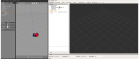
\includegraphics[scale=1]{images/imagess/6pp-rvgz.pdf}
%	\begin{tikzpicture}
%		\draw[step=1cm,gray,very thin] (0,0) grid (13,6);
%	\end{tikzpicture} 
	\caption{Gazebo and Rviz Window}
	\label{fig:Gazebo and Rviz Window}
\end{figure}
\hspace{1.27cm}
\textbf{\figureautorefname{ \ref{fig:Gazebo and Rviz Window}}}, the Gazebo robot simulation software will be used to simulate the robot, sensor and the surrounding environment. The RVIZ is used as a visualization tool. RVIZ allows us to visualize and verify the incoming data from the ROS messages. In this project, RVIZ is used to visualize the Occupancy Grid Map, Robot Model, Robot trajectory -etc.\par












\subsection{Path Planning A*}
\hspace{1.27cm}
A* algorithm is one of the path search algorithm that is widely used in many fields. In the mobile robotic field, the algorithm is used for searching the path in a robot navigation task. In this project, the A* algorithm is used to search the path for the mobile robot. The information that is given to the algorithm are the start point (robot current position), goal point (desired point to move to), and the occupancy grid map (which contain the free space and the occupied space of the environment).





















\subsubsection{Occupancy Grid Map}
\hspace{1.27cm}
Occupancy grid map is one of many pieces of information that are required for the mobile robot for navigation tasks such as path planning, navigation, environment map, and localization.\par
\hspace{1.27cm}
Occupancy grid map represents the environment in square grid cells. Each of grid cells is represented as either an occupied cell or a free cell according to the calculation of the binary probability value. \textbf{\figureautorefname{ \ref{fig:Occupancy Grid Map}}}, Occupancy Grid Map is a 2D map is a large set that contains a probability value in every cell. The cell representation as:
\begin{itemize}
	\item \textbf{Occupied cell} by probability value of (1) with black color
	\item \textbf{Free cell} by a probability value of (0) with white color
\end{itemize}
With the assumption of that the cell is either occupied or free, each probability value contained in each cell are independent, and the surrounding environment is static. Occupancy grid maps are fine-grained grids defined over the continuous space of locations and often used after solving the SLAM problem by some other means and taking the resulting path estimates for granted. \textbf{\tableautorefname{ \ref{Table: Occupancy Grid Map Properties}}} is ROS properties of Occupancy Grid Map.\par

\begin{figure}[ht]
	\centering
	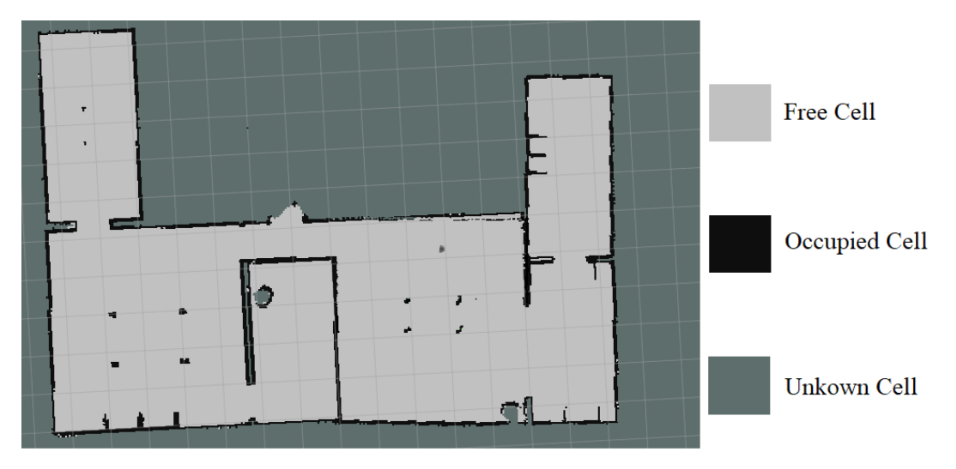
\includegraphics[scale=1]{images/imagess/6pp-pathplan_ogm.eps} 
	\caption{Occupancy Grid Map}
	\label{fig:Occupancy Grid Map}
\end{figure}
% Figure Image =============================================================================

% Table ====================================================================================
\begin{table}[ht]
    \begin{center}
		\caption{Occupancy Grid Map Properties (\cite{rosocm})}
		\label{Table: Occupancy Grid Map Properties}
		\begin{tabular}{p{0.3\linewidth}  p{0.6\linewidth}}
		ROS message & Definition \\
		\hline
        header                   & Timestamp and frame id \\
        nav\_msgs/MapMetaData    & Contain the map's resolution (m/cell), width (cell), height (cell) and origin (0,0) \\
        int8[] data              & Contain the array of probability value of map \\
        %\hline
        \ChangeRT{1.5pt} 
       \end{tabular}
  \end{center}
\end{table}
% Table ====================================================================================


\break
\hspace{1.27cm}
\textbf{\figureautorefname{ \ref{fig:Occupancy Grid Map Cell Value}}}, SLAM start with the initialization of an empty cell grid. Each cell has an address in the grid and its size is determined by the algorithm or user assign value. Then, the empty grid is filled with probability value to represent the obstacle in the environment where the robot can not traverse on.\par
\begin{figure}[ht]
	\centering
	
\includegraphics[scale=1]{images/imagess/6pp-ocm-cell-value.pdf}
%	\begin{tikzpicture}
%		\draw[step=1cm,gray,very thin] (0,0) grid (6,6);
%		\draw[step=1cm,gray,very thin] (7,0) grid (13,6);
%	\end{tikzpicture} 
	\caption{Occupancy Grid Map Cell Value}
	\label{fig:Occupancy Grid Map Cell Value}
\end{figure}










\subsubsection{A* Algorithm}
\hspace{1.27cm}
A* algorithm is an algorithm that based on the heuristic method. A* is the optimal best-first search algorithm. A* calculates the travel cost to the neighbor node from the current node. Node with the lowest cost to travel to is chosen.\par
The cost function is:
\begin{equation}
F(n)=G(n)+H(n)
\end{equation}

Where:
\begin{itemize}
	\item {\makebox[1cm]{\(F(n)\)\hfill} is the total cost of node path}
	\item {\makebox[1cm]{\(G(n)\)\hfill} is the exact distance from the starting node to the current node}
	\item {\makebox[1cm]{\(H(n)\)\hfill} is the estimation distance from the current node to the ending node}
	\item {\makebox[1cm]{\(n\)\hfill} is the node}

%	\item \(F(n)\) is the total cost of node path
%	\item \(G(n)\) is the exact distance from the starting node to the current node
%	\item \(H(n)\) is the estimation distance from the current node to the ending node. (Heuristic part of the cost function, meaning it is a guess)
%	\item \(n\) is the node
\end{itemize}

\hspace{1.27cm}
From SLAM, we obtain the occupancy grid like in figure shown below. \textbf{\figureautorefname{ \ref{fig:Occupancy Grid Map Example}}}, Each cell in the grid have its own address and the occupied value depending on SLAM. Let the origin address of the grid be in the top left corner, same as the occupancy grid map SLAM.\par
\begin{figure}[ht]
	\centering
	
\includegraphics[scale=1]{images/imagess/6pp-ocm-cell-exmpl.pdf}
%	\begin{tikzpicture}
%		\draw[step=1cm,gray,very thin] (0,0) grid (6,6);
%	\end{tikzpicture} 
	\caption{Occupancy Grid Map Example}
	\label{fig:Occupancy Grid Map Example}
\end{figure}


\hspace{1.27cm}
\textbf{\figureautorefname{ \ref{fig:Astar starting point and ending point}}}, The white cell represents the space where the robot can move and the black cell represents the space where the robot can not move. Which mean, the starting point and the ending point have to be on chosen on the white cell address.\par
\begin{figure}[ht]
	\centering
	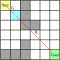
\includegraphics[scale=1]{images/imagess/6pp-ocm-start-goal.pdf}
%	\begin{tikzpicture}
%		\draw[step=1cm,gray,very thin] (0,0) grid (6,6);
%	\end{tikzpicture} 
	\caption{Astar starting point and ending point}
	\label{fig:Astar starting point and ending point}
\end{figure}


In A* cell, the cell contain 4 information, which are:
\begin{itemize}
	\item Address
	\item \(F\) value
	\item \(G\) value
	\item \(H\) value
\end{itemize}
\break
$\bullet$ \textbf{$G(n)$ value}\par
\hspace{1.27cm}
In \textbf{\figureautorefname{ \ref{fig:Euclidean Distance of G value}}}, to calculate the value of \(G(n)\) the exact distance from the starting point to the current node, we can use the Euclidean distance formula:\par

\begin{figure}[ht]
	\centering
	\includegraphics[scale=1]{images/imagess/6pp-eud-g.pdf}
%	\begin{tikzpicture}
%		\draw[step=1cm,gray,very thin] (0,0) grid (6,3);
%	\end{tikzpicture} 
	\caption{Euclidean Distance of G value}
	\label{fig:Euclidean Distance of G value}
\end{figure}
\begin{equation}
	d(a,b)^2 = (x_b - x_a)^2 + (y_b - y_a)^2
\end{equation}
\begin{equation}\label{eq:PP_euclidean_dis}
	d(a,b) = \sqrt{(x_b - x_a)^2 + (y_b - y_a)^2}
\end{equation}
Where:
\begin{itemize}
	\item {\makebox[2cm]{\(d(a,b)\)\hfill} is the distance from point a to point b}
	\item {\makebox[2cm]{\(x_a\), \(x_b\)\hfill} are the cell address of a and b in x-axis}
	\item {\makebox[2cm]{\(y_a\), \(y_b\)\hfill} are the cell address of a and b in y-axis}
	
%	\item \(d(a,b)\) is the distance from point a to point b
%	\item \(x_a\) and \(x_b\) is the cell address of a and b in x-axis
%	\item \(y_a\) and \(y_b\) is the cell address of a and b in y-axis
\end{itemize}

\break
$\bullet$ \textbf{$H(n)$ value}\par
\hspace{1.27cm}
In \textbf{\figureautorefname{ \ref{fig:Euclidean Distance of H value}}}, to calculate the value of \(H(n)\) the estimation distance from the current node to the ending node, we can use the Euclidean distance formula same as the \ref{eq:PP_euclidean_dis}. The value \(H(n)\) is the Heuristic part of the cost function, meaning it can be a guess value. Thus, in coding the square root can be dropped for the performance optimization.\par

\begin{figure}[ht]
	\centering
	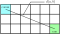
\includegraphics[scale=1]{images/imagess/6pp-eud-h.pdf}
%	\begin{tikzpicture}
%		\draw[step=1cm,gray,very thin] (0,0) grid (6,3);
%	\end{tikzpicture} 
	\caption{Euclidean Distance of H value}
	\label{fig:Euclidean Distance of H value}
\end{figure}


$\bullet$ \textbf{Parent and Child Cell} \par
\hspace{1.27cm}
In \textbf{\figureautorefname{ \ref{fig:Parent and Child Cell}}}, each cell has child cell and parent cell. Parent cell is a cell where the current node state is land on. The Child cell is the 8 neighbor cells around the parent cell.\par

\begin{figure}[ht]
	\centering
	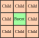
\includegraphics[scale=1]{images/imagess/6pp-par-chld.pdf}
%	\begin{tikzpicture}
%		\draw[step=1cm,gray,very thin] (0,0) grid (3,3);
%	\end{tikzpicture} 
	\caption{Parent and Child Cell}
	\label{fig:Parent and Child Cell}
\end{figure}

$\bullet$ \textbf{Initialize} \par
\hspace{1.27cm}
At start, the current node state is set to the start cell. The $H(n)$ and $G(n)$ of the cell is calculated using the \ref{eq:PP_euclidean_dis}. The $F(n)$ is the sum of the $G(n)$ and $H(n)$ \textbf{\figureautorefname{ \ref{fig:Start Point F,G,H}}}. Create 2 lists: Open list and Closed List.\par

\begin{itemize}
	\item Open List contains the cell which the cost value is yet to be calculated or traversed pass.
	\item Closed List contains the cell which the cost value is calculated or traversed pass or block by the obstacle.
\end{itemize}

Starting by adding the start cell to the Open List. After calculate the cost value, move it to the Closed List.

\break
\begin{figure}[ht]
	\centering
	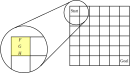
\includegraphics[scale=0.85]{images/imagess/6pp-start-cost.pdf}
%	\begin{tikzpicture}
%		\draw[step=1cm,gray,very thin] (0,0) grid (6,6);
%	\end{tikzpicture} 
	\caption{Start Point $F(n),G(n),H(n)$}
	\label{fig:Start Point F,G,H}
\end{figure}

$\bullet$ \textbf{Current state transition} \par
\hspace{1.27cm}
The $F(n),G(n),H(n)$ of the child cell to the parent cell is calculated (ignore the block cell) and add those to the Open List. If the $F(n)$ value of the child cell is the smallest of every cell, the current cell state is transit to that child cell, and it becomes the parent cell to the other. This action is loop until the goal point is found (the goal point is added to the Closed List). Then, backtracking the path from the goal to start as shown in \textbf{\figureautorefname{ \ref{fig:Current state transition}}}.\par

\begin{figure}[ht]
	\centering
	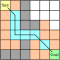
\includegraphics[scale=0.85]{images/imagess/6pp-transistion.pdf}
%	\begin{tikzpicture}
%		\draw[step=1cm,gray,very thin] (0,0) grid (6,6);
%	\end{tikzpicture} 
	\caption{Current state transition}
	\label{fig:Current state transition}
\end{figure}


$\bullet$ \textbf{A* pseudo-code} \par

\textbf{\tableautorefname{ \ref{Table: A* Pseudo-code}}} shows the pseudo-code for the A* algorithm. \textbf{\figureautorefname{ \ref{fig:A* Flowchart}}} shows the flowchart of the A* algorithm. Input data for the algorithm are: Occupancy Grid Map, Start node and Goal node. Output data for the algorithm is Pathway.







\begin{table}[ht]
	\caption{A* Pseudo-code}
	\label{Table: A* Pseudo-code}
	\begin{algorithm}[H]
	\SetAlgoLined
	\KwData{Occupancy Grid Map, Start, Goal}
	\KwResult{Path}
	INITIALIZE\;
	Let the $openList$ equal empty list of nodes\;
	Let the $closedList$ equal empty list of nodes\;
	Put the $startNode$ on the $openList$ (leave it's $f$ at zero)\;
	\While{the $openList$ is not empty}{
		Let the $currentNode$ equal the node with the least $f$ value\;
		Remove the $currentNode$ from the $openList$\;
		Add the $currentNode$ to the $closedList$\;
		\If{$currentNode$ is the goal}{
			Path Found. Backtraking to the start\;
		}
		Let the children of the $currentNode$ equal the adjacent nodes\;
		\For{each child in the children}{
			\If{child is in the $closedList$}{continue to beginning of for loop}
			$child.g$ = $currentNode.g$ + distance between child and current\;
			$child.h$ = distance from child to end\;
			$child.f$ = $child.g$ + $child.h$\;
			\If{$child.position$ is in the $openList$'s nodes positions}{\If{the $child.g$ is higher than the $openList$ node's $g$}{continue to beginning of for loop}
			Add the child to the openList}
		}
	}
	\caption{A* Pseudo-code (\cite{nicholasswift})}
	\end{algorithm}
\end{table}

\begin{figure}[ht]
	\centering
	
\includegraphics[scale=1]{images/imagess/6pp-astarfc.pdf}
	\caption{A* Flowchart}
	\label{fig:A* Flowchart}
\end{figure}
	\section{RESULT AND DISCUSSION}
\hspace{1.27cm}
The first step of our simulation is initialization. The robot model, sensors model, and simulated room are loaded into the Gazebo simulator. For the sensor's data, it is also taking into account for the noise and the uncertainty in the simulation. For the second step, we create an occupancy grid map to represent the simulated room. To do that, we use the SLAM algorithm. After the model is loaded into the simulator, we run the SLAM algorithm on the background and drive the robot manually to explore the room until SLAM create a full map. We drive the robot using keyboard input and publish its data on ("/cmd\_vel") for ROS. The result of the map obtained from SLAM is shown in \textbf{Section 7.1}. For the third step, after the map is obtained, the A* is used for finding the path from start to goal in the map. On ROS the path is published on ("/path"). The result of the path from A* is shown in \textbf{Section 7.2}. Finally, the robot controller is used to control the robot while EKF is localizing the robot pose in the map. The result of control path is shown in \textbf{Section 7.3}. \textbf{\tableautorefname{ \ref{Table: Simulation Parameters}}} and \textbf{\tableautorefname{ \ref{Table: Sensor and Algorithm Data Publication Rate for EKF}}} show the initialize parameter and the rate of data publishing.\par


%First, the robot model and the sensor model is loaded in to the Gazebo simulator. And two room models is loaded: "Map1" and "Map2". Second, the robot is driven around the room by keyboard command ("/cmd\_vel") while the SLAM algorithm is running to create the occupancy grid map ("/map"). Third, the A* is used to search the path from start to goal in the map ("/path"). Finally, the robot controller is used to control the robot while EKF is localizing the robot pose in the map. \textbf{\tableautorefname{ \ref{Table: Simulation Parameters}}} and \textbf{\tableautorefname{ \ref{Table: Sensor and Algorithm Data Publication Rate for EKF}}} show the initialize parameter and the rate of data publishing.\par


\begin{table}[ht]
	\begin{center}
		\caption{Simulation Parameters}
		\label{Table: Simulation Parameters}
		\begin{tabular}{ccc}
			Parameter                    &Value                              &Unit           \\
			\hline
			k1                           &5                                  &-              \\
			k2                           &10                                 &-              \\
			k3                           &10                                 &-              \\
			ka                           &15                                 &-              \\
			kb                           &15                                 &-              \\
			$r$                          &0.1                                &$m$            \\
			$L$                          &0.2                                &$m$            \\
			Q                            &$diag(1^2,0.52^2)\times 0.01$      &-              \\
			R                            &$diag(1^2,1^2,1^2)\times 0.01$     &-              \\
			%\hline
			\ChangeRT{1.5pt} 
		\end{tabular}
	\end{center}
\end{table}


\begin{table}[ht]
	\begin{center}
		\caption{Sensor and Algorithm Data Publication Rate for EKF}
		\label{Table: Sensor and Algorithm Data Publication Rate for EKF}
		\begin{tabular}{ccc}
			Data Publish                 &Rate             &Unit            \\
			\hline
			Encoder                      &20               &Hz              \\
			IMU                          &10               &Hz              \\
			Lidar Scan Match             &30               &Hz              \\
			EKF Fusion                   &20               &Hz              \\
			%\hline
			\ChangeRT{1.5pt} 
		\end{tabular}
	\end{center}
\end{table}



\textbf{\figureautorefname{ \ref{fig:Robot Model Simulation}}} shows the Differential Drive Wheeled Mobile Robot and Sensors (IMU, Lidar, Wheel Encoder) 3D model that is viewed inside Gazebo Simulator. \textbf{\figureautorefname{ \ref{fig:Map1 and Map2 in simulation}}} shows the 3D models of simulated rooms.

% Figure Image =============================================================================
\begin{figure}[ht]
	\centering
	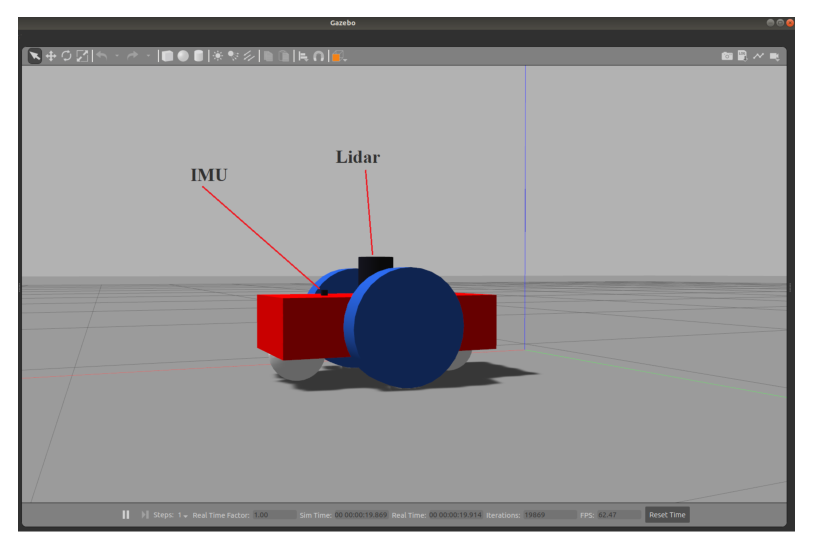
\includegraphics[scale=1]{images/imagess/3method-gazebo.eps} 
	\caption{Robot Model Simulation}
	\label{fig:Robot Model Simulation}
\end{figure}
% Figure Image =============================================================================

\begin{figure}[H]
	\centering
	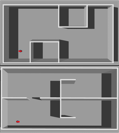
\includegraphics[scale=1]{images/imagess/7reslt-map1and2.pdf} 
	\caption{Map1 and Map2 in simulation}
	\label{fig:Map1 and Map2 in simulation}
\end{figure}



\subsection{SLAM}
% SLAM
\hspace{1.27cm}
In this section, we show the result from the SLAM algorithm of "Map1" and "Map2". First, the robot is placed in the room at the start location. Our goal is drive the robot manually to create the map. While the SLAM algorithm is running, we use keyboard input to move the robot along the green line from start to goal location. SLAM output the occupancy grid map and is visualized using RVIZ as shown in \textbf{\figureautorefname{ \ref{fig:Map1 SLAM}}} and \textbf{\figureautorefname{ \ref{fig:Map2 SLAM}}}. From the figures, the white space is the free space that allow the robot to move in while the black line is the obstacle.\par
\begin{figure}[H]
	\centering
	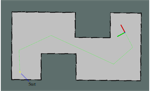
\includegraphics[scale=0.80]{images/imagess/7reslt-slam-map1.pdf}
	\caption{Map1 SLAM}
	\label{fig:Map1 SLAM}
\end{figure}

\begin{figure}[H]
	\centering
	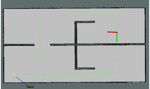
\includegraphics[scale=0.80]{images/imagess/7reslt-slam-map2.pdf}
	\caption{Map2 SLAM}
	\label{fig:Map2 SLAM}
\end{figure}
Hector SLAM algorithm build an accurate occupancy grid map from the simulated room.



\subsection{Path Planning}
\hspace{1.27cm}
In this section, we show the result of the A* path planning algorithm of "Map1" and "Map2". After the occupancy grid map from the previous section is build, we put the robot at a resting state on the start location on the map. Then we chose the goal location that we want the robot to go. The A* algorithm calculates an optimal path from the map and those 2 locations and output a trajectory of the robot to follow in brown line as in \textbf{\figureautorefname{ \ref{fig:Map1 Path Planning}}} and \textbf{\figureautorefname{ \ref{fig:Map2 Path Planning}}}. As the algorithm is in function with Heuristic function, the H value should not be overestimated.\par


%In this section, the path is searched from start to goal point using the A*. The start point is chosen to be the current pose of the robot and the goal point is where we put in the location that we want the robot to go. In the figure below, the brown line is the path that the algorithm generated.

\begin{figure}[H]
	\centering
	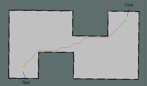
\includegraphics[scale=0.80]{images/imagess/7reslt-pp-map1.pdf}
	\caption{Map1 Path Planning}
	\label{fig:Map1 Path Planning}
\end{figure}

\begin{figure}[H]
	\centering
	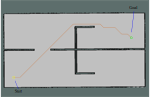
\includegraphics[scale=0.80]{images/imagess/7reslt-pp-map2.pdf}
	\caption{Map2 Path Planning}
	\label{fig:Map2 Path Planning}
\end{figure}




\subsection{Control}
\hspace{1.27cm}
In this section, we show the control of the robot path from start to goal. After the trajectory is generated from the A* from the last section, the controller is required to move the robot. The backstepping controller calculate the required linear velocity and angular velocity from the trajectory and the current position of the robot. To keep track of robot position, the EKF is used to estimated it location and feedback to the controller. For better performance, the constants variable in \textbf{\tableautorefname{ \ref{Table: Simulation Parameters}}} is manually tuned. In the \textbf{\figureautorefname{ \ref{fig:Map1 Control}}} and \textbf{\figureautorefname{ \ref{fig:Map2 Control}}}, the brown line is the path that the algorithm generated. The blue line is the path that the robot currently move. As seen in the figures, the blue line follow the brown line accurately which mean the control performance is acceptable.\par


\begin{figure}[H]
	\centering
	\includegraphics[scale=0.75]{images/imagess/7reslt-cntrl-map1.pdf}
	\caption{Map1 Control}
	\label{fig:Map1 Control}
\end{figure}

\begin{figure}[H]
	\centering
	\includegraphics[scale=0.75]{images/imagess/7reslt-cntrl-map2.pdf}
	\caption{Map2 Control}
	\label{fig:Map2 Control}
\end{figure}
	\section{CONCLUSION AND RECOMMENDATION}
\subsection{Conclusion}
\hspace{1.27cm}
In conclusion, the experiment is conducted in Gazebo simulation with the robot 3D model and sensors (wheel encoders, IMU, and Lidar). The kinematic and dynamics model of differential drive mobile robot is derived. We use algorithms:\par
\begin{itemize}
	\item \textbf{Extended Kalman Filter} for sensor fusion localization
	\item \textbf{Hector SLAM} to create the occupancy grid map
	\item \textbf{A* Path Planning} to determine the optimal pathway for the robot from starting point to goal point coming from user desired input
	\item \textbf{Backstepping} controller to control the robot motion
\end{itemize}

\hspace{1.27cm}
In static map, the A* path planning algorithm achieve a great result in generate pathway in low computational time because the cost function has the heuristic value $H$. The pathway is optimal as long as its value is not overestimated. The backsteppig controller results controlled output close to the generated pathway while the EKF give an accurate pose estimation.\par

\hspace{1.27cm}
The usage of ROS package from this project can be extended. In the robot control section, the controller can be further developed or switched between another controller. With the three sensors that is used in this project, we can add or switch with other sensors that provide a suitable data that the algorithm required. This project has produced a ROS package and framework for the differential drive mobile robot for other to test, simulate, and visualize the robot in the simulated environment. For further implementation in the real world scenario, this ROS package implement ROS topics that are ready for real devices to publish its data on. \par


%To determine the robot pose in the surrounding, the extended kalman filter algorithm for sensor fusion is used. In the simulation, we simulated three sensors: wheel encoders, IMU, and Lidar. To obtain the occupancy grid map, the hector SLAM algorithm is used. After obtain the map, we use A-star path planning algorithm to generate the optimal path from starting point to goal point coming from user desired input. The robot motion is controlled using the backstepping controller. Although the project is in simulation, it has built a groundwork for the real world implementation in the future.\par

%Conclude performance 
%	feedback control
%	SLAM
%Conclude framework ability in real system
%
%for static map all the algorithm is suitable
%ROS framework can be used for further testing
%convenience for different controller


\subsection{Recommendation}
\hspace{1.27cm}
In the future work, the project will be implemented in hardware. With hardware implementation, the algorithm required more accuracy and performance to cope with the hardware capability such as computational speed, data publishing rate, sensor noise and interference, unexpected failure, disturbance properties that have not been considered in the modeling. \par
	
	
	\section*{REFERENCES}
\addcontentsline{toc}{section}{REFERENCES}
\printbibliography[heading=none] %DON'T SHOW HEADING BECAUSE IT ALREADY SHOWN IN SECTION COMMAND
	\include{Main-pages/appendix1}
	\include{Main-pages/appendix2}
	\include{Main-pages/appendix3}
	\begin{appendices}
\section{Control and EKF}
$\bullet$ \textbf{Control}\par
\begin{lstlisting}[language=Python]
#! /usr/bin/env python

import numpy as np
import rospy
from nav_msgs.msg import Odometry
from geometry_msgs.msg import Point, Pose,Quaternion, Twist, Vector3
from tf.transformations import euler_from_quaternion, quaternion_from_euler

def angnorm(theta):
	if theta>0:
		if theta>np.pi:
			theta = (2*np.pi-theta)*(-1)

	if theta<0:
		if theta*(-1)>np.pi:
			theta = (2*np.pi-(-theta))*(-1)
	return theta

class backstp_contrl:

def __init__(self,k1,k2,k3,ka,kb,m,r,b,Iner):
	self.k1   = k1
	self.k2   = k2
	self.k3   = k3
	self.ka   = ka
	self.kb   = kb
	self.m    = m
	self.r    = r
	self.b    = b
	self.Iner = Iner

def error(self,qr,qc):
	"""Calculate error from the current pose to the reference pose. return qe"""
	theta = qc[2,0]
	
	T = np.array([[np.cos(theta),np.sin(theta),0],
					[-np.sin(theta),np.cos(theta),0],
					[      0       ,     0       ,1]]) # (3X3)
	
	e = qr - qc
	return T.dot(e) # (3X1)

def controlkinematic(self,qe,vr,wr):
	""" Control Algorithm for Kinematic, return : vc, wc"""
	return ((vr*np.cos(qe[2,0]))+self.k1*qe[0,0]),(wr+(self.k2*vr*qe[1,0])*(self.k3*np.sin(qe[2,0])))

def controldynamics(self,vdotref,wdotref):
	""" Control Algorithm for Dynamics, z1= vref-vcur , z2 = wref-wcur, return : tua1c, tua2c """
	return 1/2*((self.m*self.r*(vdotref+self.ka*z1))+((2*self.r*self.Iner/b)*(wdotref+self.kb*z2))),1/2*((self.m*self.r*(vdotref+self.ka*z1))-((2*self.r*self.Iner/b)*(wdotref+self.kb*z2)))

sq = 0
def odm_callback(msg):
	global sq
	# Find Current Pose
	x = msg.pose.pose.position.x
	y = msg.pose.pose.position.y
	qq = msg.pose.pose.orientation
	ol = [qq.x,qq.y,qq.z,qq.w]
	(rl,pt,yw)=euler_from_quaternion(ol)
	qc = np.array([[x],[y],[yw]])
	
	# Find Desired Pose
	xRef,yRef,theta_ref,vr,wr,ydot,xdot,vdotref,wdotref = ref_8(sq)
	qr = np.array([[xRef],[yRef],[theta_ref]])
	
	# Control init for each trajectory
	#contl = backstp_contrl(0.7,20,20,100,3000,4,0.1,0.26,2.5) # For ref_circle
	contl = backstp_contrl(0.7,20,20,100,3000,4,0.1,0.26,2.5) # For ref_8
	
	# Find error and control
	qe = contl.error(qr,qc)
	vc,wc = contl.controlkinematic(qe,vr,wr)
	
	# Print some output
	rospy.loginfo("thetaref = "+str(theta_ref)+"       thetac = "+str(qc[2,0]))
	
	# Publish to ROS
	tw_p = rospy.Publisher("/robotros_test/cmd_vel", Twist, queue_size = 50)
	Twm = Twist()
	Twm.linear.x = vc
	Twm.angular.z = wc
	tw_p.publish(Twm)
	sq += 1

def main():

	rospy.init_node('BS_Ctrl')
	rospy.Subscriber('/ground_truth/state',Odometry, odm_callback)
	rospy.spin()

if __name__=='__main__':
	main()

\end{lstlisting}


$\bullet$ \textbf{EKF}\par
\begin{lstlisting}[language=Python]
#! /usr/bin/env python

import numpy as np
import time

import rospy
from nav_msgs.msg import Odometry
from sensor_msgs.msg import Imu
import tf
from geometry_msgs.msg import Point, Pose, Quaternion, Twist, Vector3, Pose2D


class EKF_node(object):
def __init__(self):

	self.xest = np.array([[0],[0],[0]])
	self.pest = np.eye(3)
	self.z = np.array([[0],[0],[0]])
	
	self.loopr = rospy.Rate(20)
	
	rospy.Subscriber('/pose2D',Pose2D, self.read_lidr)
	
	self.pub = rospy.Publisher("/odom_filter", Odometry, queue_size = 50)

def read_lidr(self,msg):
	yy = msg.theta
	if yy < 0:
	yy = np.pi + (np.pi+yy)
	self.z = np.array([[msg.x],[msg.y],[yy]])
	Ts = 0.05

	# input calculate
	noise = np.diag([1.,np.deg2rad(30.)])**2
	v = 1
	w = 0.5
	u = np.array([v,w]) #+ noise.dot(np.random.rand(2,1))
	
	# jacob F
	yaw = self.xest[2,0]
	jF = np.array([[1.,0,-v*np.sin(yaw)*Ts],[0,1.,v*np.cos(yaw)*Ts],[0,0,1.]])
	
	# prediction
	Q = np.diag([0.1,0.1,np.deg2rad(1.)])**2
	F = np.array([[1.,0,0],[0,1.,0],[0,0,1.]])
	B = np.array([[Ts*np.cos(self.xest[2,0]),0],[Ts*np.sin(self.xest[2,0]),0],[0,Ts]])
	xpred = F.dot(self.xest)+B.dot(u)
	ppred = jF.dot(self.pest.dot(jF.T)) + Q
	
	# update
	R = np.diag([0.1,0.1,0.1])**2
	y = self.z - xpred
	jH = np.diag([1.,1.,1.])
	s = (R + jH.dot(ppred.dot(jH.T)))
	K = ppred.dot((jH.T).dot(np.linalg.inv(s)))
	self.xest = xpred + K.dot(y)
	self.pest = (np.eye(3) - K.dot(jH)).dot(ppred)

if __name__ == '__main__':

	rospy.init_node('ekf_locl_fusion')
	nod = EKF_node()
	
	while not rospy.is_shutdown():
	odom_broadcaster = tf.TransformBroadcaster()
	odom = Odometry()
	odom_quat = tf.transformations.quaternion_from_euler(0,0,nod.xest[2,0])
	odom_broadcaster.sendTransform((nod.xest[0,0],nod.xest[1,0],0.),odom_quat,rospy.Time.now(),"base_link_filter","odom_filter")
	odom.header.frame_id = "filter_odom"
	odom.pose.pose = Pose(Point(nod.xest[0,0],nod.xest[1,0],0.),Quaternion(*odom_quat))
	odom.child_frame_id = "filter_base_link"
	nod.pub.publish(odom)
	nod.loopr.sleep()
\end{lstlisting}
\end{appendices}
	
	%Back cover
	
\includepdf[pages={1}]{cover/coverback}
\end{document}